\documentclass[11pt, a4paper]{article}
\usepackage[english]{babel}
\usepackage{amsmath}
\usepackage{amssymb}
\usepackage{placeins}
\usepackage{empheq}
\usepackage{hhline}
\usepackage{graphicx}
\usepackage{subcaption}
\usepackage{amsthm}
\usepackage[binary-units=true]{siunitx}
\usepackage{mathrsfs}
\usepackage[multiple]{footmisc}
\usepackage{bbold}
\usepackage{lscape}
\usepackage{setspace}
\usepackage{a4wide}
\usepackage{color}
\usepackage{tikz, pgfplots}
\pgfplotsset{compat=1.9}
\usetikzlibrary{arrows.meta}
\usetikzlibrary{calc}
\usetikzlibrary{shapes,arrows,backgrounds}
\usepackage{algcompatible}
\usepackage{algorithm}
\usepackage{algpseudocode}
\usepackage{varwidth}
\usepackage[inline]{enumitem}
\usepackage{dsfont}
\usepackage{fullpage}
\usepackage{multirow}
\usepackage[Symbol]{upgreek}
\usepackage{wrapfig}
\usepackage[pdfborder={0 0 0}]{hyperref}
\usepackage{url}
\usepackage{authblk}
\usepackage[normalem]{ulem}
\usepackage{hyperref}
\hypersetup{
    colorlinks=true,       % false: boxed links; true: colored links
    linkcolor=blue,       % color of internal links
    citecolor=blue,       % color of links to bibliography
    filecolor=black,       % color of file links
    urlcolor=black,         % color of external links
    pdffitwindow=true,
    pdfpagelayout=SinglePage
}
\usepackage{cite}


\newcommand{\Sha}{\mbox{\usefont{T2A}{\rmdefault}{m}{n}\CYRSH}}
\newcommand{\fig}{\figurename \ }
\makeatletter
\newcommand{\algo}{\ALG@name \ }
\makeatother
\newcommand{\tableau}{\tablename \ }
\newcommand{\red}[1]{\textcolor{red}{#1}}
\renewcommand{\vec}[1]{\boldsymbol{#1}}
\newcommand{\secondOrderTensor}[1]{\underline{\boldsymbol{#1}}}
\newcommand{\tensor}[1]{\underline{\underline{\boldsymbol{#1}}}}
\newcommand{\green}[1]{\textcolor{green}{#1}}
\newcommand{\blue}[1]{\textcolor{blue}{#1}}
\newcommand{\im}{\text{i}}
\newcommand{\Der}[2]{\frac{\mathrm{d} #1}{\mathrm{d} #2}}
\newcommand{\DDer}[2]{\frac{\mathrm{d^2} #1}{\mathrm{d} #2^2}}
\newcommand{\partDer}[2]{\frac{\partial #1}{\partial #2}}
\newcommand{\partder}[2]{\partial_{#2} #1}
\newcommand{\dist}[2]{\text{dist}\left( #1, #2 \right)}
\newcommand{\diag}[1]{\text{diag}\left( #1\right)}
\newcommand{\Reynolds}{\text{Re}}
\newcommand{\delete}[1]{\textcolor{red}{\sout{#1}}}
\newcommand{\bigOhNothation}[1]{\mathcal{O}\left( #1 \right)}
\newcommand{\realSet}{\mathds{R}}
\newcommand{\spaceOfRealVectors}[1]{\realSet^{#1 \times 1}} 
\newcommand{\spaceOfRealMatrices}[2]{\realSet^{#1 \times #2}} 

\theoremstyle{remark}
\newtheorem{remark}{Remark}
\newcommand{\rem}{Remark \ }
\newtheorem{theorem}{Theorem}[section]
\newcommand{\thm}{Theorem \ }
\newtheorem{lemma}[theorem]{Lemma}
\newcommand{\lem}{Lemma \ }

\definecolor{vert}{rgb}{0.3,0.7,0}
\renewcommand{\green}[1]{\textcolor{vert}{#1}}
\DeclareMathOperator{\cotan}{cotan}
\DeclareMathOperator{\sinc}{sinc}
\DeclareMathOperator*{\argmax}{argmax}

\newcommand{\Mymp}{\mathbin{\smash{%
\raisebox{0.35ex}{%
            $\underset{\raisebox{0.5ex}{$\textcolor{vert}{\smash +}$}}{\smash-}$%
            }%
        }%
    } %
}

\newcommand{\Mypm}{\mathbin{\smash{%
\raisebox{0.35ex}{%
            $\underset{\raisebox{0.5ex}{$\textcolor{vert}{\smash -}$}}{\smash+}$%
            }%
        }%
    } %
}
\newcommand{\ohm}{\Upomega}
\newcommand{\rot}[1]{\nabla \times #1}
\newcommand{\divergence}[1]{\nabla \cdot #1}
\newcommand*{\I}{\imath}


\begin{document}
\renewcommand{\arraystretch}{1.1}

\title{Optimization of the Navier-Stokes Solver on Distributed Adaptive Quad-/Oc-tree Grids}

\author{
Raphael Egan
}

\maketitle

\begin{abstract}
The optimization-based modifications brought to the Navier-Stokes solver on distributed adaptive Quad-/Oc-tree are presented, summarized and explained. The modifications are validated by comparing the original and optimized solvers on the flow past a sphere/disk in 3D/2D with advection of a passive scalar. The gain of performance is reported, discussed and illustrated with respect to user-defined numerical parameters for some applications.
\end{abstract}


\section{Summary of the modifications}
\label{sec:summary}
The typical usage of the Navier-Stokes solver follows the flow chart from \fig \ref{fig:flow_chart}. The modifications brought to the solver target different parts of such a typical flow chart but can be divided into various categories depending on their scope of interest and/or on the typical subpart of the flowchart that they aim to optimize. 

\begin{figure}
\centering
% Define block styles
\tikzstyle{decision} = [diamond, draw, fill=blue!20, 
    text width=4.5em, text badly centered, node distance=3cm, inner sep=0pt]
\tikzstyle{block} = [rectangle, draw, fill=blue!20, 
    text width=10em, text centered, rounded corners, minimum height=3em]
\tikzstyle{line} = [draw, -latex']
\tikzstyle{cloud} = [draw, ellipse,fill=red!20, node distance=5.5cm,
    text width=12em, text centered, minimum height=3em]
\begin{tikzpicture}[node distance = 2.5cm, auto]
    % Place nodes
    \node [block] (input) {read user's input(s)};
    \node [block, below of=input, text width=16em] (init) {initialize all solver's parameters to input(s) or default values.\\ Set $n = 0$, $t_{0} = t_{\text{start}}$, and $\Delta t_{0} = t_{1}-t_{0}$};
    \node [cloud, right of=init, node distance=7.5cm] (flags) {set exportation flags, exportation parameters, grid update flags, grid update parameters, etc.};
    \node [right of=flags, node distance=4.8cm] (top_right_anchor){};
    \node [decision, text width=6.em, below of=init] (loop_start) {is $t_{n}$ equal to $t_{\text{end}}$?};
    \node [decision, right of=loop_start, node distance=3.8cm] (first_step) {is $n>0$?};
    \node [block, right of=first_step, node distance=4.5cm] (get_new_dt) {get $\Delta t_{n} = t_{n+1}-t_{n}$};
    \node [block, below of=get_new_dt, node distance=2.cm] (grid_update) {update grid if desired.};
    \node [block, below of=first_step, node distance=3.5cm] (export_state) {export solver's state if desired and if requried};
    \node [block, below of=export_state, node distance=2.5cm] (viscosity_step) {solve for $\mathbf{v}^{\star}$ (BC $\sim \nabla \Phi_{n+1}$)};
    \node [block, below of=viscosity_step, node distance=2.5cm] (projection_step) {solve for $\Phi_{n+1}$ ($-\Delta \Phi_{n+1} = \divergence{\mathbf{v}^{\star}}$)};
    \node [decision, right of=projection_step, node distance=5.5cm, text width = 6em] (exit_sub_loop) {$\Phi_{n+1}$ converged or max \# subiterations reached?};
    \node [below of=projection_step, node distance=2.4cm](under_projection_step){};
    \node [left of=under_projection_step, node distance=8em, label=above right:{\red{Inner loop for convergence of $\Phi_{n+1}$}}] (lower_left_subloop_corner){};
    \node [above of=exit_sub_loop, node distance=3.6cm](above_exit_subloop){};
    \node [right of=above_exit_subloop, node distance=2.6cm] (upper_right_subloop_corner){};
    \begin{scope}[on background layer]
     \draw[black,fill=yellow!40,rounded corners=1ex] (lower_left_subloop_corner) rectangle (upper_right_subloop_corner);
    \end{scope}
    \node [block, below of=projection_step, node distance=3.5cm] (interp_velocity) {interpolate $\mathbf{v}_{n+1}$ at nodes,\\ calculate $p_{n+1}$};
    \node [block, below of=interp_velocity, node distance=2.8cm, text width=14em] (exportation) {if desired and if required, export relevant data. \\ Update $t_{n} \leftarrow t_{n} + \Delta t_{n}$ and $n \leftarrow n+1$};
    \node [block, left of=exportation, node distance=6.cm, text width=6em] (stop) {clear memory and stop};
    % Draw edges
    \path [line] (init) -- (loop_start);
    \path [line] (loop_start) -- node {no}(first_step);
    \path [line] (loop_start) -| node [above left] {yes}(stop);
    \path [line] (first_step) -- node {yes}(get_new_dt);
    \path [line] (get_new_dt) -- (grid_update);
    \path [line] (first_step) -- node {no}(export_state);
    \path [line] (grid_update) |- (export_state);
    \path [line] (export_state) -- (viscosity_step);
    \path [line] (viscosity_step) -- (projection_step);
    \path [line] (projection_step) -- (exit_sub_loop);
    \path [line] (exit_sub_loop) |- node [above left] {no}(viscosity_step);
    \path [line] (exit_sub_loop) |- node [below right] {yes}(interp_velocity);
    \path [line] (interp_velocity) -- (exportation);
    \path [line] (exportation) -| (loop_start);
    \path [line] (input) -- (init);
    \path [line,dashed] (input) -- (flags);
    \path [line,dashed] (flags) -- (top_right_anchor) |- (grid_update);
    \path [line,dashed] (flags) -- (top_right_anchor) |- (export_state);
    \path [line,dashed] (flags) -- (top_right_anchor) |- (exportation);
\end{tikzpicture}
\caption{\label{fig:flow_chart}typical flow chart for the usage of the one-phase Navier-Stokes solver.}
\end{figure}


\subsection{Modifications or additions of general interest}
\label{subsec:general_interest}
The following modifications and additions were made to the \verb|casl_p4est| library. They may be of general interest to all users.
\begin{itemize}
 \item Restart tools were developped to enable the possibility to export/load an exact given state defined as the association of a given \verb|p4est| object and a set of relevant node-, cell- or even face-sampled data fields. The state can be reloaded with a different number of MPI processes than when written on disk, and the relevant data is re-scattered to the new global orderings in a way that is consistent with the data layout when exported.
 \item The interpolations tools (from nodes, cell-centers or faces) were generalized to allow the interpolation of several fields \emph{simultaneously}, under the same desired interpolation scheme. This is especially relevant when interpolating several node-sampled fields from one grid to a unique set of desired nodes, with the same interpolation procedure: for instance, when setting node values of a newly updated grid based on node values of the former grid. Another relevant example is the interpolation of node-sampled vector fields, for which this approach can cut down the costs by the number of vector components (\textit{e.g.,} calculations of semi-lagrangian trajectories).\\
 Such an approach reduces the number of lookups in the hierarchy and, more importantly, cuts down the number of more costly operations per point in the set (like the calculations of non-initialized direct neighbors in quadratic node interpolation, or the resolution of least-square systems in cell or face cases) by the number of fields to be interpolated simultaneously. \\
 The user must be \textbf{careful} when using such a feature with cell-centered or face-centered fields as boundary conditions are required and queried in such a case: \emph{currently, this generalization assumes that all fields share the exact same boundary conditions for interpolation of cell- or face-sampled data}.
 \item A similar generalization was done for the calculation of second derivatives of several node-sampled fields simultaneously, in \verb|my_p4est_node_neighbors|.
 \item Basic core function of the \verb|matrix_t| class (solving least-square systems, calculations of Choleski factorizations, etc.) were modified accordingly to allow the resolution of linear systems involving possibly more than one right-hand-side vector.
 \item The classes \verb|my_p4est_faces_t|, \verb|my_p4est_hierarchy_t|, \verb|my_p4est_node_neighbors_t|, \break \verb|my_p4est_navier_stokes_t| were augmented with \verb|memory_estimate| functions that return an estimate of the raw number of bytes that the corresponding objects require. Similarly, a function was added to \verb|my_p4est_tools.c| in order to estimate the memory requirement of \verb|my_p4est_brick_t| objects. Except for \verb|my_p4est_navier_stokes_t| objects, these functions assess the memory requirement associated with every single MPI process and an \verb|MPI_allreduce| call is required afterwards to estimate the global memory requirement. The estimates measure the raw data requirements, hence they are not exact but still very representative. They were designed to make a distinction between the growing memory requirement due to an increasingly finer grid and a possible memory leak. The memory estimate for the \verb|my_p4est_nodes_t| data structures would be very helpful, however not straightforward to implemented (and not implemented yet in \verb|p4est|).
 \item Two functions \verb|nodes_are_equal| and \verb|ghosts_are_equal| were added to \verb|p4est_utils| to check equality between two \verb|p4est_nodes_t| and between two \verb|p4est_ghost_t| structures, respectively. The two functions check that every single item is identical, ordered in the same way and that the local and global indices are identical. The tests are processed locally, an \verb|MPI_allreduce| call is required afterwards to test equality globally.
 \item A function \verb|index_of_node| was developped and added to \verb|p4est_utils|. This function takes any node and its tree index as defined within \verb|p4est|\footnote{In \texttt{p4est}, a node is defined as a specific \texttt{p4est\_quadrant\_t} object whose \texttt{level} field is assigned the value \texttt{P4EST\_MAX\_LEVEL} (which is defined as \texttt{P4EST\_QMAX\_LEVEL+1}, hence the unambiguous distinction with any actual quadrant). The regular \emph{logical} coordinates \texttt{x}, \texttt{y}, \texttt{z} and the tree index of the considered node make its localization unambiguous and robust (no floating point arithmetics error is possible).}\textsuperscript{,}\footnote{To ensure that the binary search finds any given point that exists, the node and its tree index \emph{must be canonicalized} before being passed to \texttt{index\_of\_node}. The \texttt{static} qualifier of the \texttt{p4est\_node\_canonicalize} function from \texttt{my\_p4est\_nodes.c} was removed so that it can be used from another context. This ensures consistency between the considered node and the nodes as they were defined when the \texttt{p4est\_nodes\_t} data structure was assembled. It is \emph{critical} if the node lies exactly on a tree boundary and its owning tree is not clear. Even if only one tree is used, the node must be \emph{clamped} inside the domain.} to perform a binary search based on the tree and Morton indices that are used to sort the nodes internally by \verb|p4est_nodes_t|. If the given node actually exists in the current forest, the function returns a positive answer along with its local node index. If the considered node does not exist and/or does not belong to the \verb|p4est_nodes_t| data structure, a negative answer is returned.\\ 
 Hence, this function finds any existing node indexed by the local partition in $\mathcal{O}\left( \log\left( N \right) \right)$ operations without the need of constructing a local hierarchy object, which was the typical former approach.
\end{itemize}

\subsection{Inner loop optimization}
\label{subsec:inner_loop_optimization}
The following modifications were implemented in order to optimize the possible inner loop for convergence of the Hodge variable $\Phi_{n+1}$ (see \fig \ref{fig:flow_chart}).
\begin{itemize}
 \item The Poisson solver for face-sampled (vector) fields \verb|my_p4est_poisson_faces_t| was modified in order to store in memory all \verb|P4EST_DIM| matrices that it builds. Previously, those matrices (and the corresponding preconditioned Krylov solvers) were built and destroyed immediately after the solve-step for the velocity component that was currently treated, one after the other. This impeded the possible reuse of the (exact same) Krylov solvers within such a possible inner loop, introducing an overhead cost for recalculating the very same matrices and solvers as previsouly destroyed. This modification applies for the interface-stress-balanced two-phase flows solver.
 \item The \verb|solve_viscosity| and \verb|solve_projection| functions within the Navier-Stokes solver now allow the user to possibly feed them with valid face-based and cell-based Poisson solvers and/or to retrieve them from the object for possible reuse. If the corresponding parameter is \verb|NULL| on input, the functions build the solvers internally and return them to the calling environment (instead of destroying it, right away). Therefore, the user can now possibly reuse the solvers within such an inner loop, avoiding the cost of re-assembling the linear system and re-building preconditioners.
 \item These functions also now allow the user to specify the kinds of Krylov solver and preconditioners they wish to use for their application. The default values for these fields are what used to be hard-coded internally, \textit{i.e.} a BiConjugate Gradient Stabilized (\verb|BiCGStab|) solver with Successive Over-Relaxation (\verb|SOR|) for the preconditioner. While \verb|BiCGStab| is the only safe choice for the solvers in the most general context (given that interface boundary conditions might break matrices' symmetries), there are better preconditioners to use than \verb|SOR| in general.
 \item All relevant backtraced semi-lagrangian points in \verb|solve_viscosity| are calculated \emph{simultaneously}, instead of considering faces dimension by dimension. This cuts down the number of calls to interpolation procedure by \verb|P4EST_DIM|. For that purpose, a capability to calculate trajectories of several lists of points at once has been added (to minimize the number of calls to \verb|trajectory_from_np1_to_n(m1)| which all used up to \verb|5*P4EST_DIM| interpolation procedures). In summary the number of calls to interpolation tools was cut down by a factor \verb|P4EST_DIM*PEST_DIM| which was terribly slow if the node neighbors were not initialied. All former relevant functions for semi-lagrangian backtracing of faces along one single Cartesian direction now call this generalized function (although they should be considered outdated from now on).
 \item All relevant backtraced semi-lagrangian points are stored in memory and calculated only once per inner loop for $\Phi_{n+1}$-convergence (\textit{i.e.,} not recalculated in case of subiterations).
\end{itemize}

\subsection{General time-stepping optimization in absence of grid update}
\label{subsec:general_time_stepping}
The following modifications were implemented in order to optimize time-stepping in case of absence of modifications in the computational grid (either enforced/desired by the user or as a result of the regular grid-update procedure if it reaches a conclusion that no grid update nor any modification to the levelset were made). 
\begin{itemize}
 \item The cell- and face-based Poisson solvers were modified to allow a simple update of the constant coefficient term. If the grid is not modified, the solvers from the previous time step are almost ready to be re-used: their memory allocation is still valid, their sparsity is unchanged and most off-diagonal terms are unchanged, only the terms affected by the constant coefficient need to be updated (most are on the diagonal of the matrices, but not necessarily all of them). The objects now allow to keep track of such states and update only the relevant terms within the matrices, which avoids costly reconstructions of the entire matrices.\\
 The \verb|update_from_tn_to_tnp1| function from the Navier-Stokes solver now returns a boolean value that is true if the solvers for viscosity and projection steps can be used again in the future. This flag can be true if and only if the grid has not been changed (nor its partitioning) and if the levelset has not been modified either. Otherwise, the solvers must be deleted and reconstructed!
 \item In case of no grid update, only the set of grid-defining objects corresponding to time step $n$ is kept in memory. The corresponding pointers associated with $\left(n-1\right)$-objects simply point to the $n$-objects. This was meant to ensure the re-usability of face- and cell-solvers for the following time step: since the grid is not modified, we keep it as such, we do not create a new one and we make the $\left(n-1\right)$-pointers point to the $n$-object. Data management was modified to avoid deletion of $\left( n-1 \right)$-objects if they happen to point to $n$-objects.
 \item No expensive cell-to-cell nor face-to-face interpolations are executed when no modification to the computational grid was made. 
\end{itemize}

\subsection{Non-restricted optimization of the solver}
\label{subsec:nonrestricted_optimization_of_the_solver}
The following modifications target general optimizaton of several distinct parts within the Navier-Stokes solver.
\begin{itemize}
 \item The node neighbors are \emph{initialized} right after the finalization of a new distributed grid and of the corresponding new distributed nodes. This speeds up significantly all calculations querying access to the node neighbors like the calculations of spatial first or second derivatives. Previously, the node neighbors were initialized only for data extension over the interface (in presence of an interface in the computational domain) at the very end of every time step.
 \item All \verb|P4EST_DIM| spatial second derivatives along Cartesian axes of the \verb|P4EST_DIM| velocity components (at nodes) at times $n$ and $\left( n-1 \right)$ are now stored in memory in order to accelerate all quadratic interpolation of velocity fields (required in the calculation of semi-lagrangian trajectories \emph{and} in the definition of the right-hand sides of the viscosity step).
 \item The solver now allows the user to choose between two different time steps satisfying either a \emph{global} or \emph{local} CFL condition. The global CFL requirement defines the time step as  
 $$\Delta t = \dfrac{\text{CFL}\, \min_{\Omega}\left( \Delta x, \Delta y, \Delta z \right)}{\max_{\Omega} \left\| \mathbf{v}_{n+1}\right\|_{2}}$$ 
 whereas, the local CFL requirement defines it as
 $$\Delta t = \text{CFL} \min_{\Omega}\left( \dfrac{\Delta x}{\left\| \mathbf{v}_{n+1}\right\|_{2}}, \dfrac{\Delta y}{\left\| \mathbf{v}_{n+1}\right\|_{2}}, \dfrac{\Delta z}{\left\| \mathbf{v}_{n+1}\right\|_{2}}\right)$$ 
 which ensures that the CFL conditions is satisfied locally everywhere. The former definition might be much more restrictive than the latter in simulations where the largest velocities are found in the coarsest regions and vice versa, \textit{e.g.} developing or laminar flows past a sphere, channel flows, etc. 
 \item For the very first iteration of the iterative grid-update procedure, the grid-related data structures are no longer built except for the a copy of the raw grid. Similarly, the node-sampled voriticy does not go through a dummy interpolation and the levelset function either if it is not modified.
 \item The iterative grid-update procedure no longer builds the ghost layer and the hierarchy at every iteration, except in case of smoke advection associated with smoke-based grid refinement since they are required for the resolution of the advection equation in this case. The final ghost layer is built only once, after completion of the grid update procedure.\\ 
 The construction of a ghost layer and the corresponding hierarchy were significant time-consuming parts of every grid update iteration. Regarding the ghost cells, they are relevant in this context for the sole purpose of identifying T-junction nodes that happen to lie exactly on the partition's border without being owned by itself. As for the hierarchy, it was used for easily finding any possible local node (owned or not by the current partition).\\
 Putting in balance the solver's behavior with the extra cost of creating a ghost layer and the extra \verb|MPI| communication it created, I decided to allow the grid update to miss the (supposedly few) such border T-junction nodes that are not owned. The rationale is that 
 \begin{itemize}
  \item a 2:1 grid balance is still enforced anyways so that such misses should not be too detrimental eventually;
  \item the iterative grid update procedure will very likely change the grid partition and such missed nodes could as well be indexed by the partition in the next iteration.
 \end{itemize}
 The usage of the costly-to-build hierarchy was replaced by the \verb|index_of_node| binary-search capability detailed in subsection \ref{subsec:general_interest}: if the node actually exists, its index is found in $\mathcal{O}\left( \log\left( N \right)\right)$ operations.
 \item When refining with smoke, the smoke advection is not recalculated after the grid update procedure if the 2:1 grid balancing operations turned out to leave the grid unchanged. Instead the current valid \verb|smoke_np1| vector is simply re-scattered to the new vector layout.
 \item The number of operations in the procedure to tag quadrant with their refining or coarsening status was minimized, and break statements are used to exit loops as soon as the (final) result is known.
\end{itemize}

\subsection{General optimization-related intel for the \texttt{casl\_p4est} developers}
I attempted to further optimize the execution time by changing all core linear algebra functions from the \verb|matrix_t| class to \verb|CBLAS| and \verb|LAPACKE| functions (mainly \verb|cblas_dgemv|, \verb|cblas_dgemm|, \verb|LAPACKE_dpotrf| and \verb|LAPACKE_dgels|). However, those core linear algebra functions are called as such when evaluating local moving-least-square interpolations and it turns out that the linear systems to be solved are not large enough to observe a significant improvement from the optimized cache management done under the hood by those optimized library. Actually, it even makes the execution slightly slower. I commented the modifications in the corresponding files in case someone else wants to ever try it again in the future...
\section{Incomplete modifications}

There was a mistake in the treatment of Neumann wall-boundary conditions on velocity components when an interface is close, this has been fixed. Starting from that observation, I decided to implement a feature to activate a possibility to account for second derivatives of Hodge variables in case of Neumann boundary conditions. If the corresponding flag is activated, those second derivatives are estimated, otherwise a value of $0$ is substituted. 

However, it became overwhelmingly complicated and I had to give up by the end of the assembly of linear system and of its right-hand side. Therefore, the task is not completed yet but it is documented! As of now, only the unactivated flag value is acceptable!

\section{Showing unchanged behavior besides runtime}
First, the performance results are shown in 2D and 3D based on test cases that are designed to show an unchanged solver's behavior, yet a significant gain in runtime due to better computing strategies: namely the more efficient iterative grid-update procedure, calculations of semi-lagrangian backtraced points, and grouped interpolations procedure. 

These two benchmark cases run the \emph{exact} same solver configurations. No cell-/face-based poisson solver is ever re-used but disposed of after every single use. The test cases involve advection of smoke (\textit{i.e.}, a passive scalar) and adaptive refinement is triggered by distance to the interface, local vorticity and local value of the passive scalar. Therefore, the grid update procedure must be unchanged as well\footnote{In absence of refinement based on local values of a passive scalar, the ghost layers are no longer created within the iterative grid-update procedure, which can lead to a modified behavior overall because of T-junctions lying exactly on partitions' boundaries but not owned by them}. 

All runs have been processed on a machine running a dual Intel Xeon 6148 2.4 \SI{2666}{\mega\hertz} 20C CPU, with \SI{64}{\gibi\byte} DDR4.

\subsection{Flow past a cylinder}
\label{subsec:flow_past_cylinder_check}
For the two-dimensional example, we consider the flow past a static cylinder with advection of a passive scalar (smoke). The domain size is $\left[0, 32 \right]\times \left[ -8, 8\right]$. The cylinder is centered at $\left( 8, 0 \right)$ and has a radius of $r_{0} = 0.5$. The macro-mesh is made of $8$ trees along $x$ and $4$ trees along $y$ (aspect ratio of $1$ for all quadrants). The trees are refined with minimum refinement level $4$ and maximum refinement level $6$, with the following grid-refinement parameters:
\begin{itemize}
 \item the vorticity threshold value for triggering local refinement is $0.1\dfrac{\max_{\Omega}\left( \left\| \mathbf{v} \right\|_{2}\right)}{\max\left( \Delta x, \Delta y \right)}$;
 \item a uniform band of $2$ finest grid cells is enforced on either side of the surface of the cylinder;
 \item the threshold value for triggering smoke-based refinement is $0.5$.
\end{itemize}


The boundary conditions are 
\begin{itemize}
 \item homogeneous Dirichlet boundary condition at the inlet (left wall) and homogeneous Neumann on all other walls for the pressure;
 \item homogeneous Neumann for pressure on the surface of the cylinder;
 \item Dirichlet boundary condition $\mathbf{u} = u_{0}\mathbf{e}_{x} = \mathbf{e}_{x}$ for the velocity components on all walls but the outlet (right wall) on which homogeneous Neumann is enforced;
 \item homogeneous Dirichlet boundary condition for $\mathbf{u}$ on the surface of the cylinder (no-slip);
 \item the smoke is released into the computational domain by a unit Dirichlet boundary condition on part of the inlet wall: $x = 0$, $\left| y\right| < 0.5$.
\end{itemize}
The initial condition for the velocity field is $\left.\mathbf{u}\left( \mathbf{x}, t\right)\right|_{t = 0} = u_{0}\mathbf{e}_{x} = \mathbf{e}_{x}$. The initial boundary condition for the smoke is $0$ everywhere but in $\left[0, \, 2 \right]\times \left[ -1, \, 1\right]$ where it is $1$.

The mass density of the fluid is $\rho = 1$, its dynamic viscosity is set to $\mu = \dfrac{2 r_{0}\rho u_{0}}{\Reynolds} = \dfrac{1}{\Reynolds}$ where $\Reynolds = 350$ in the following tests. The simulations were run using $8$ cores with a second-order semi-lagrangian advection scheme, the CFL number is enforced to be smaller than or equal to $1$ (global criterion) until a simulation time of $400$ for a total number of $9950$ time steps. The number of grid cells grows from around $9,500$ to about $35,000$ as the K\'{a}rm\'{a}n street develops. 

\subsubsection*{Results and performances}
The original solver completed the simulation in \SI{1}{\hour}\,\SI{41}{\minute}\,\SI{45}{\second} while the optimized solver completed the very same task with the exact same numerics in \SI{56}{\minute}\,\SI{19}{\second}, that is a \textbf{44.64\% gain}. The only difference observed in the exported results relates to slight differences in the very first residuals for the Hodge variable in $6$ out of $9,950$ time steps. These slight differences can be explained by a modification brought to the Moving-Least-Square cell-interpolation procedure that intends to make the procedure more robust and less sensitive to the grid size (comparison of dimensionally consistent double-precision real numbers). The results are illustrated in \fig \ref{fig:forces_flow_past_cylinder_check_unchanged} and \fig \ref{fig:grid_and_smoke_flow_past_cylinder_check_unchanged}.

\begin{figure}
  \centering
  \includegraphics[width=0.49\textwidth]{./results/flow_past_cylinder_smoke/reference/force_history.pdf}
  \includegraphics[width=0.49\textwidth]{./results/flow_past_cylinder_smoke/optimized_run/force_history.pdf}
 \caption{\label{fig:forces_flow_past_cylinder_check_unchanged} history of the non-dimensional force components for $300 < t < 400$ in the simulation described in subsection \ref{subsec:flow_past_cylinder_check}. Top: original solver; bottom: optimized solver.} 
\end{figure}

\begin{figure}
  \centering
  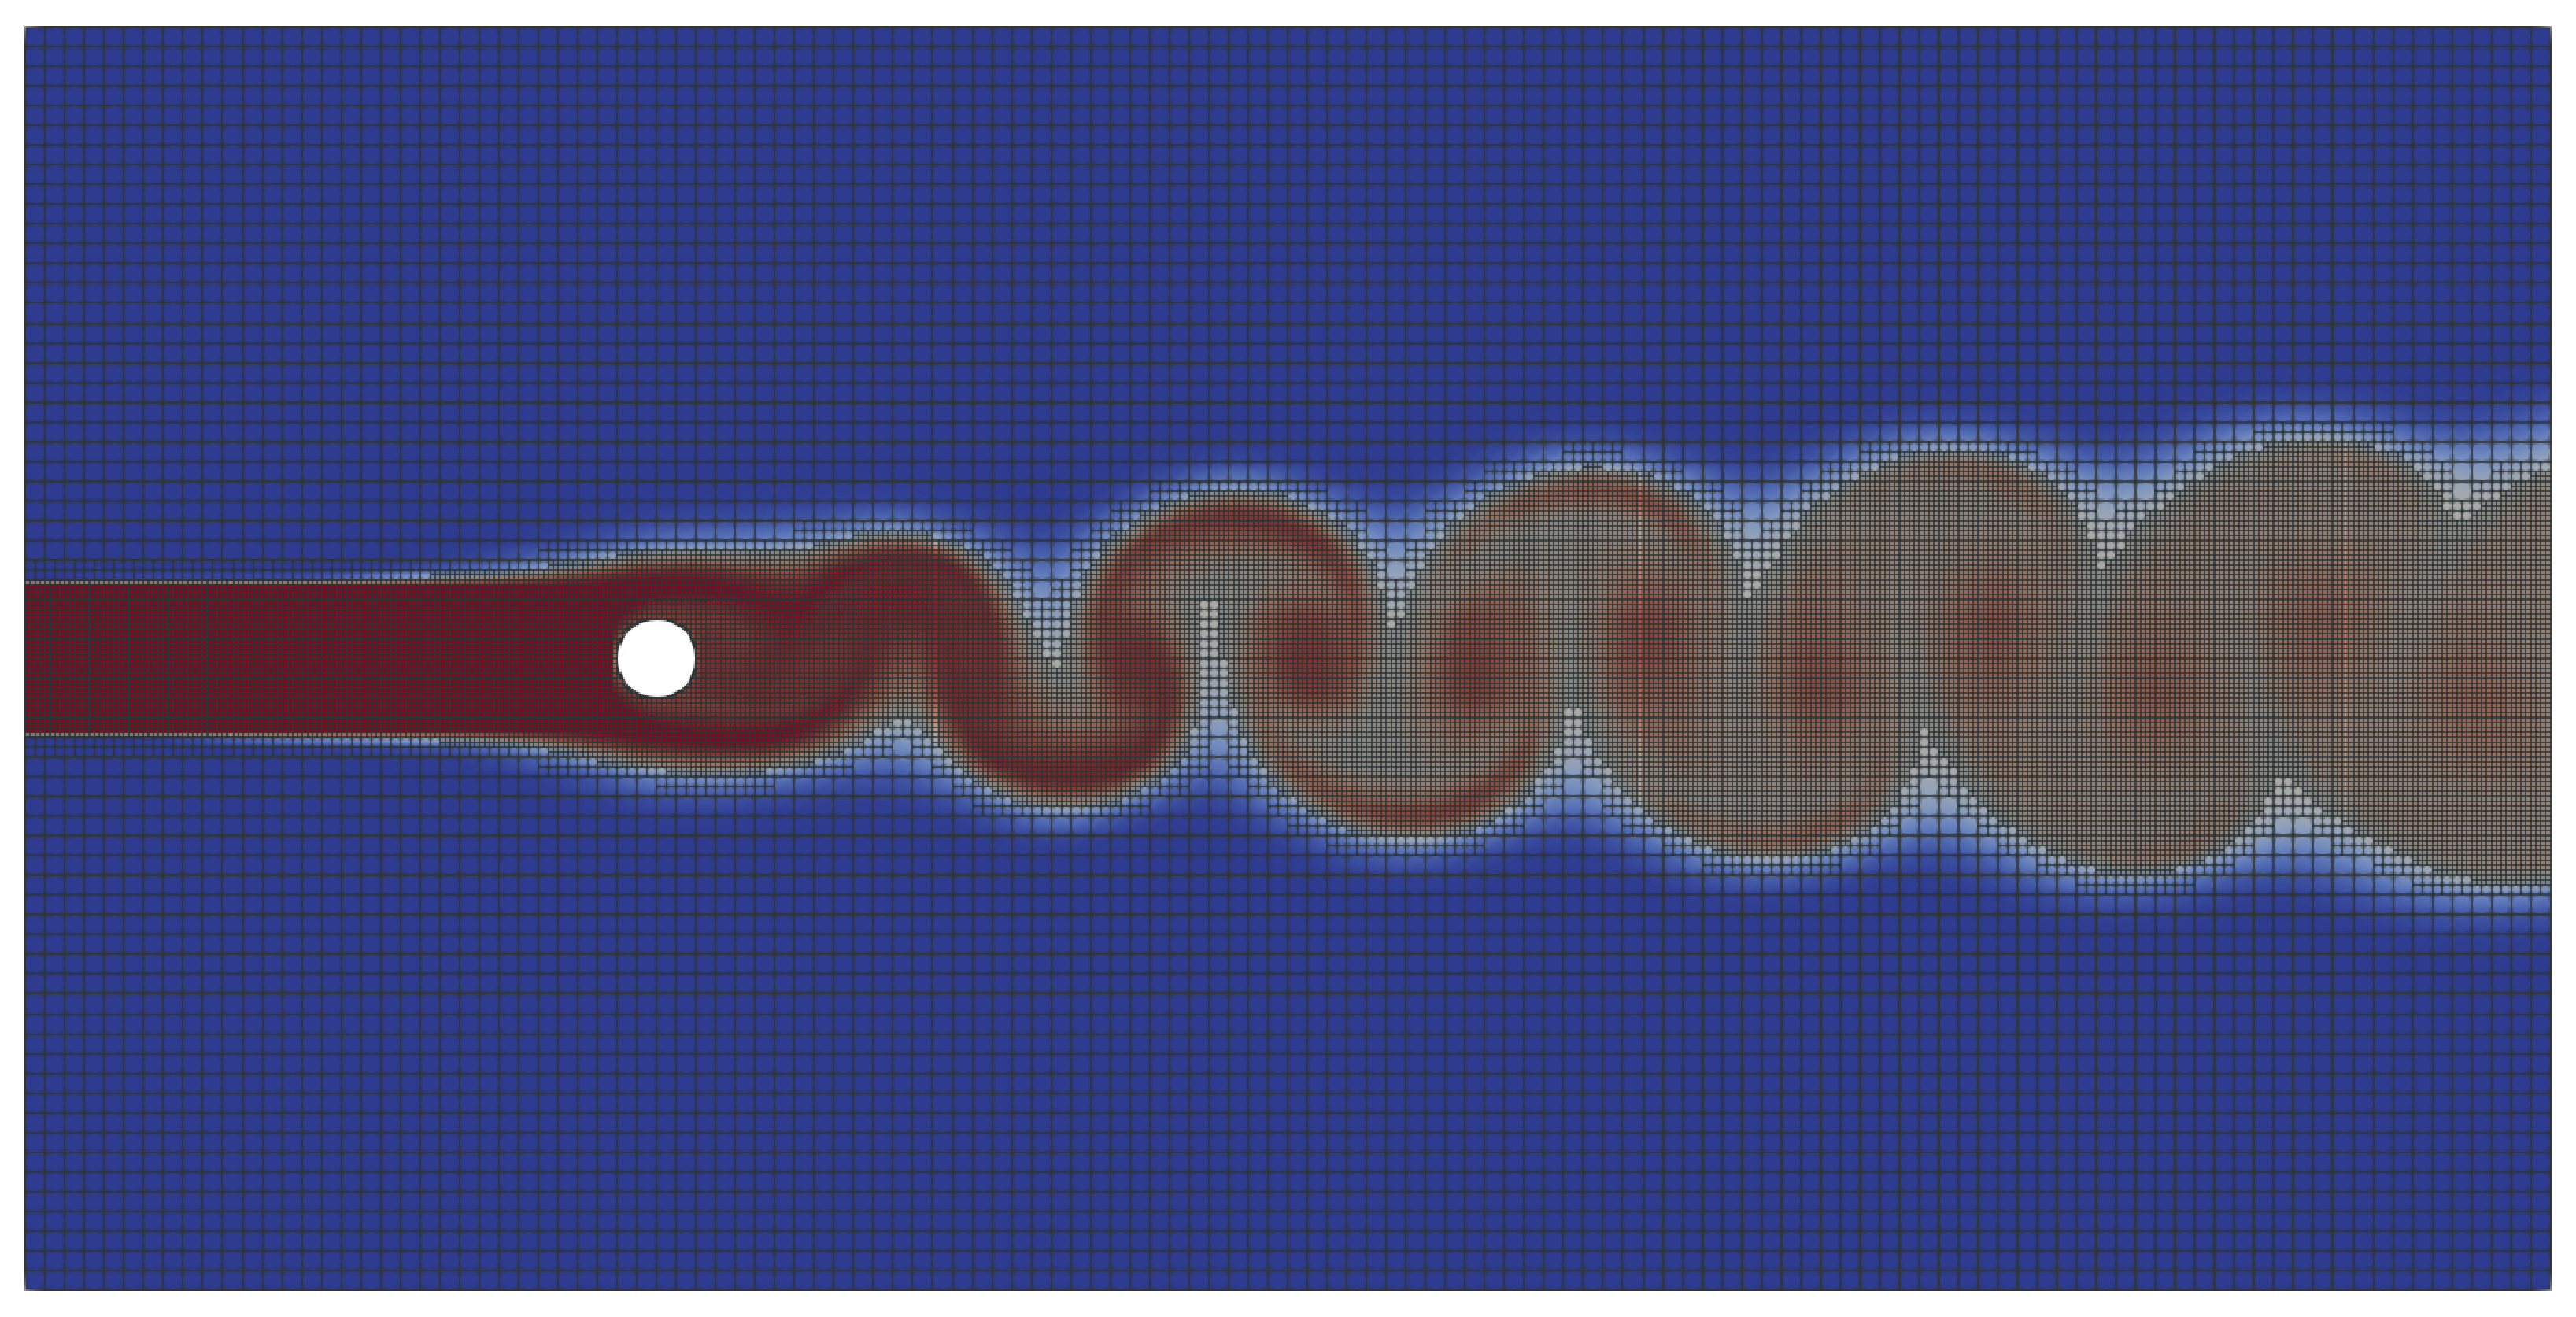
\includegraphics[width=0.95\textwidth]{./figures/flow_past_cylinder/check_unchanged_behavior/original_grid_and_smoke_t_is_300.pdf} \\
  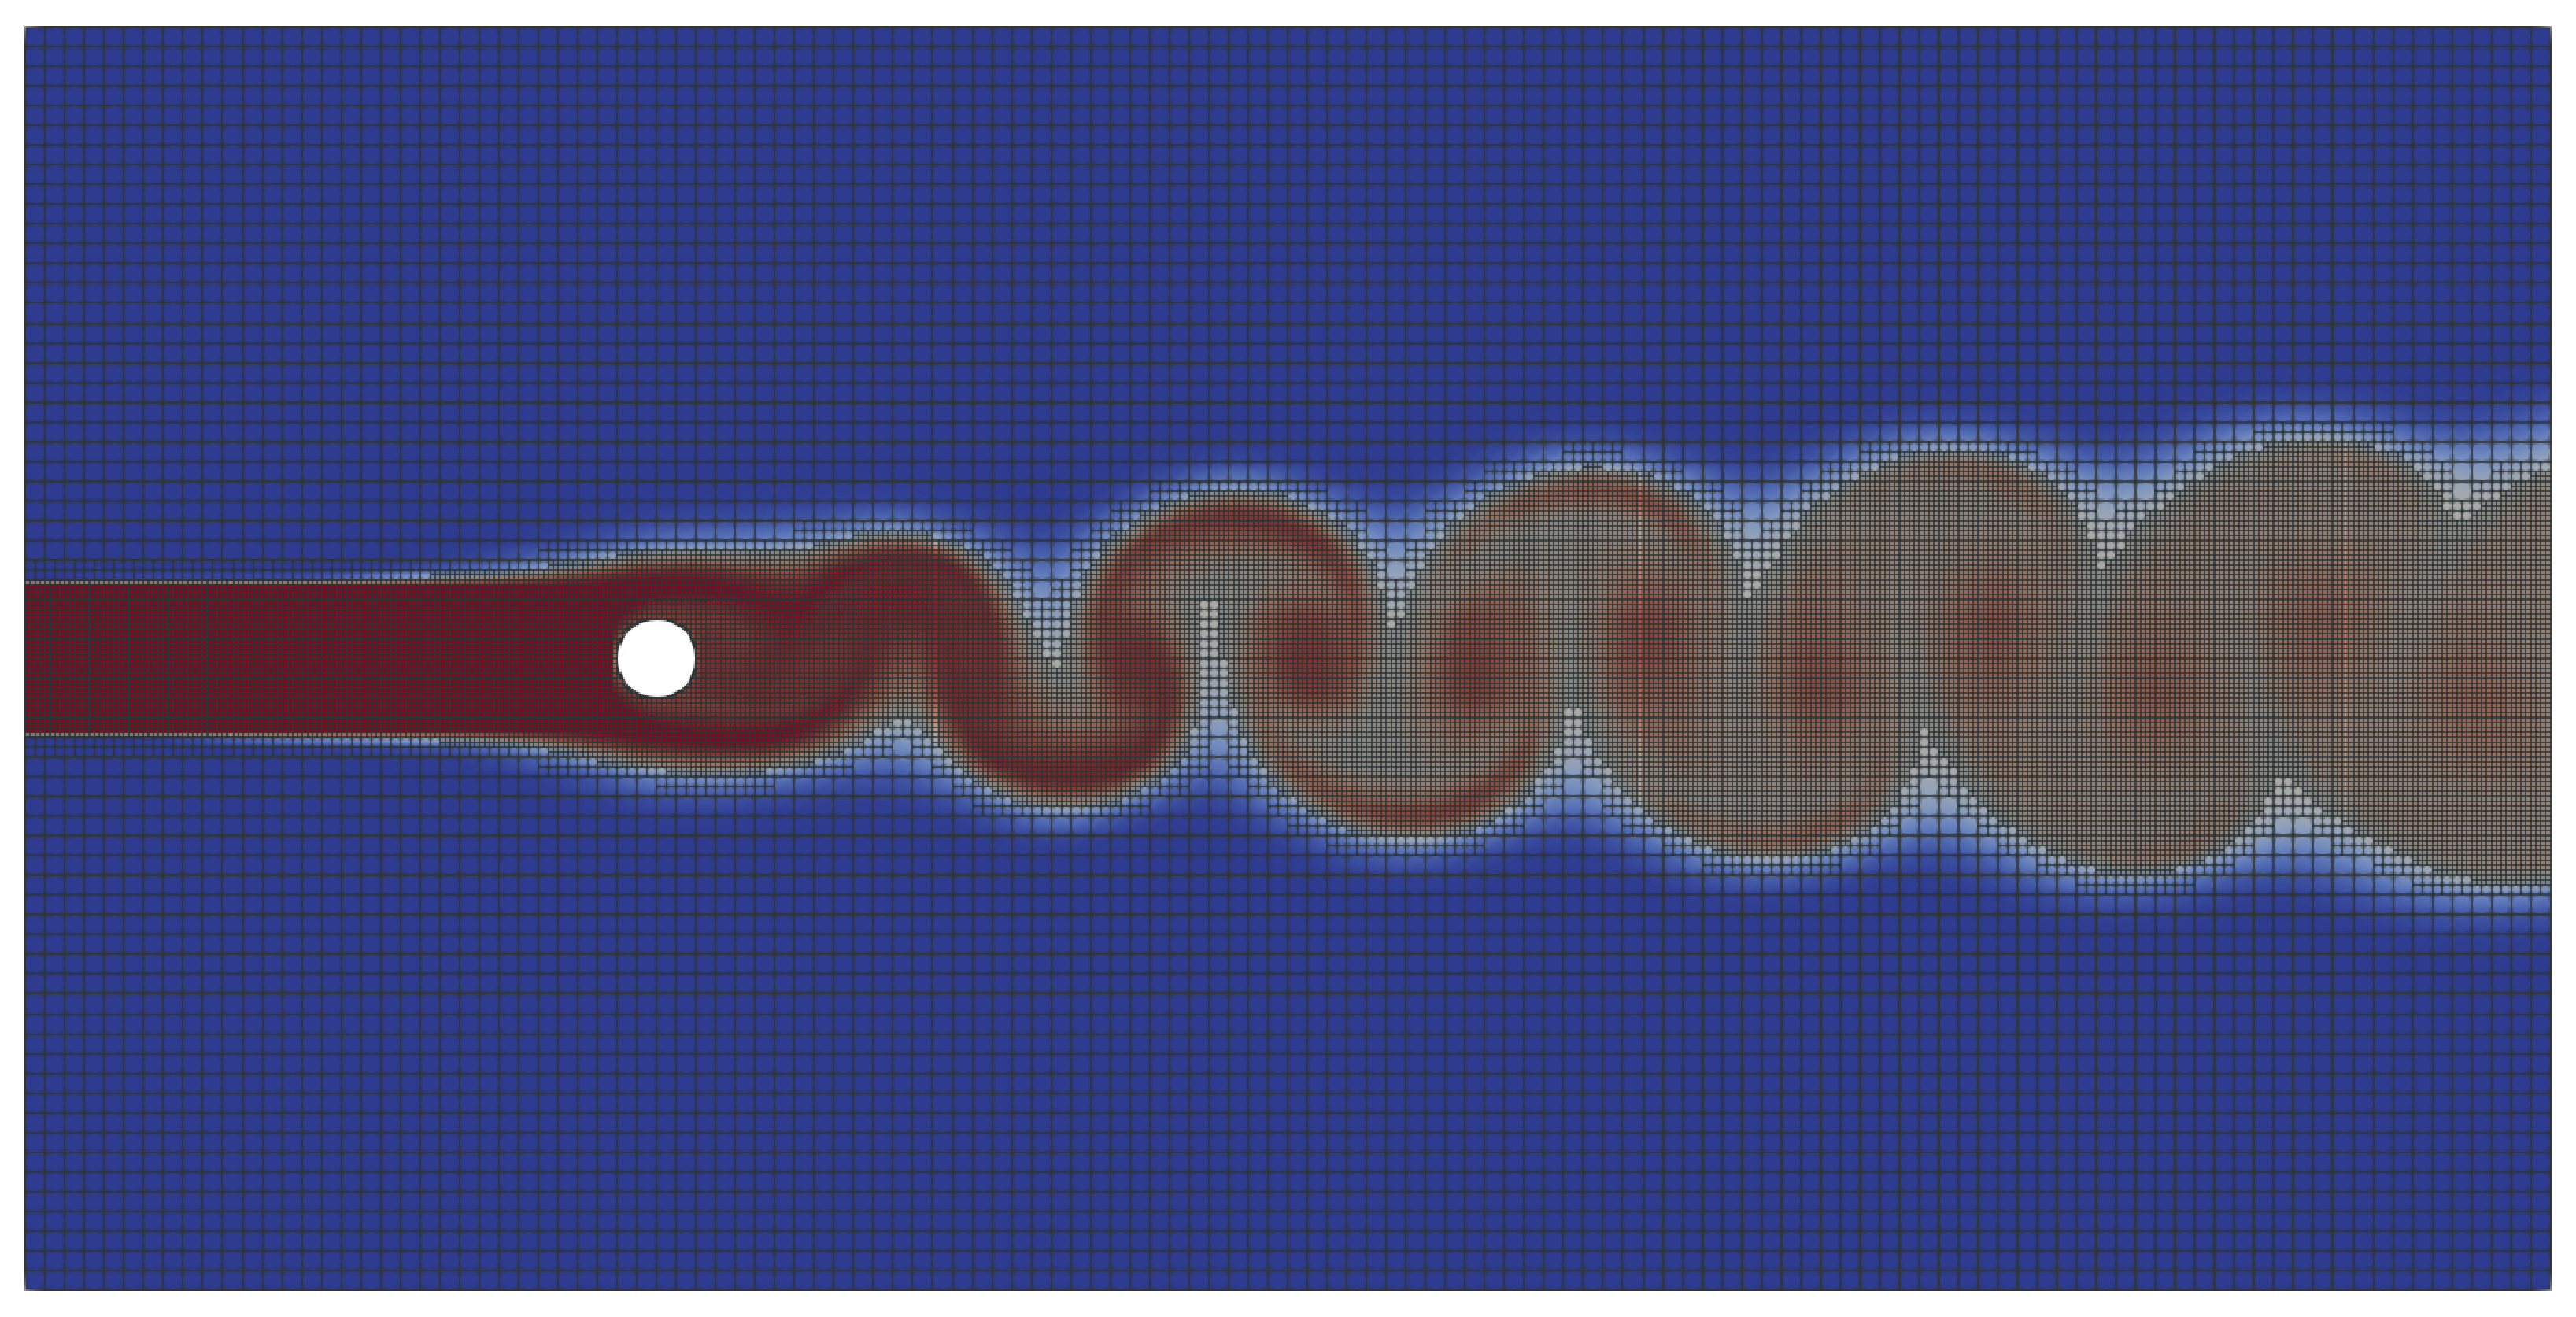
\includegraphics[width=0.95\textwidth]{./figures/flow_past_cylinder/check_unchanged_behavior/optimized_grid_and_smoke_t_is_300.pdf}
 \caption{\label{fig:grid_and_smoke_flow_past_cylinder_check_unchanged} computational grid and color map of the advected smoke for $t = 300$ in the simulation described in subsection \ref{subsec:flow_past_cylinder_check}. Top: original solver; bottom: optimized solver.}
\end{figure}



\subsection{Flow past a sphere}
\label{subsec:flow_past_sphere_check}
For the three-dimensional example, we consider the flow past a static sphere, with advection of a passive scalar (smoke). The domain size is $\left[0, 32 \right]\times \left[ -8, 8\right] \times \left[ -8, 8\right]$. The sphere is centered at $\left( 8, 0, 0 \right)$ and has a radius of $r_{0} = 1$. The macro-mesh is made of $8$ trees along $x$, $4$ trees along $y$ and $4$ trees along $z$ (aspect ratio of $1$ for all quadrants). The trees are refined with minimum refinement level $4$ and maximum refinement level $6$, with the following grid-refinement parameters:
\begin{itemize}
 \item the vorticity threshold value for triggering local refinement is $0.1\dfrac{\max_{\Omega}\left( \left\| \mathbf{v} \right\|_{2}\right)}{\max\left( \Delta x, \Delta y \right)}$;
 \item a uniform band of $2$ finest grid cells is enforced on either side of the surface of the cylinder;
 \item the threshold value for triggering smoke-based refinement is $0.5$.
\end{itemize}


The boundary conditions are 
\begin{itemize}
 \item homogeneous Dirichlet boundary condition at the inlet ($x = 0$ wall) and homogeneous Neumann on all other walls for the pressure;
 \item homogeneous Neumann for pressure on the surface of the sphere;
 \item Dirichlet boundary condition $\mathbf{u} = u_{0}\mathbf{e}_{x} = \mathbf{e}_{x}$ for the velocity components on all walls but the outlet ($x = 32$ wall) on which homogeneous Neumann is enforced;
 \item homogeneous Dirichlet boundary condition for $\mathbf{u}$ on the surface of the sphere (no-slip);
 \item the smoke is released into the computational domain by a unit Dirichlet boundary condition on part of the inlet wall: $x = 0$, $\sqrt{y^2 + z^2} < 0.4$.
\end{itemize}
The initial condition for the velocity field is $\left.\mathbf{u}\left( \mathbf{x}, t\right)\right|_{t = 0} = u_{0}\mathbf{e}_{x} = \mathbf{e}_{x}$. The initial boundary condition for the smoke is $0$ everywhere but in $\left\{ 0 \leq x \leq 2\right\} \bigcap \left\{ \sqrt{ y^2 + z^2} < 0.4\right\}$ where it is $1$.

The mass density of the fluid is $\rho = 1$, its dynamic viscosity is set to $\mu = \dfrac{2 r_{0}\rho u_{0}}{\Reynolds} = \dfrac{2}{\Reynolds}$ where $\Reynolds = 350$ in the following tests. The simulations were run using $36$ cores with a second-order semi-lagrangian advection scheme, the CFL number is enforced to be smaller than or equal to $1$ (global criterion) until a simulation time of $200$ for a total of $3,852$ time steps. The number of grid cells grows from around $558,280$ to about $700,000$ as the wake develops behind the sphere. 

\subsubsection*{Results and performances}

The original solver completed the simulation in \SI{1}{\day}\,\SI{11}{\hour}\,\SI{12}{\minute}\,\SI{56}{\second} while the optimized solver completed the very same task with the exact same numerics in \SI{23}{\hour}\,\SI{12}{\minute}\,\SI{41}{\second}, that is a \textbf{34.09\% gain}. The only difference observed in the exported results relates to slight differences in the very first residuals for the Hodge variable in $6$ out of $3,852$ time steps. These slight differences can be explained by a modification brought to the Moving-Least-Square cell-interpolation procedure that intends to make the procedure more robust and less sensitive to the grid size (comparison of dimensionally consistent double-precision real numbers). The results are illustrated in \fig \ref{fig:forces_flow_past_sphere_check_unchanged} and \fig \ref{fig:grid_and_smoke_flow_past_sphere_check_unchanged}. 

\begin{figure}
  \centering
  \includegraphics[width=0.49\textwidth]{./results/flow_past_sphere_smoke/reference/force_history.pdf}
  \includegraphics[width=0.49\textwidth]{./results/flow_past_sphere_smoke/optimized_run/force_history.pdf}
 \caption{\label{fig:forces_flow_past_sphere_check_unchanged} history of the non-dimensional force components for $100 < t < 200$ in the simulation described in subsection \ref{subsec:flow_past_sphere_check}. Top: original solver; bottom: optimized solver. (The graphs for $C_{\mathrm{D}, y}$ and $C_{\mathrm{D}, z}$ overlap)} 
\end{figure}

\begin{figure}
  \centering
  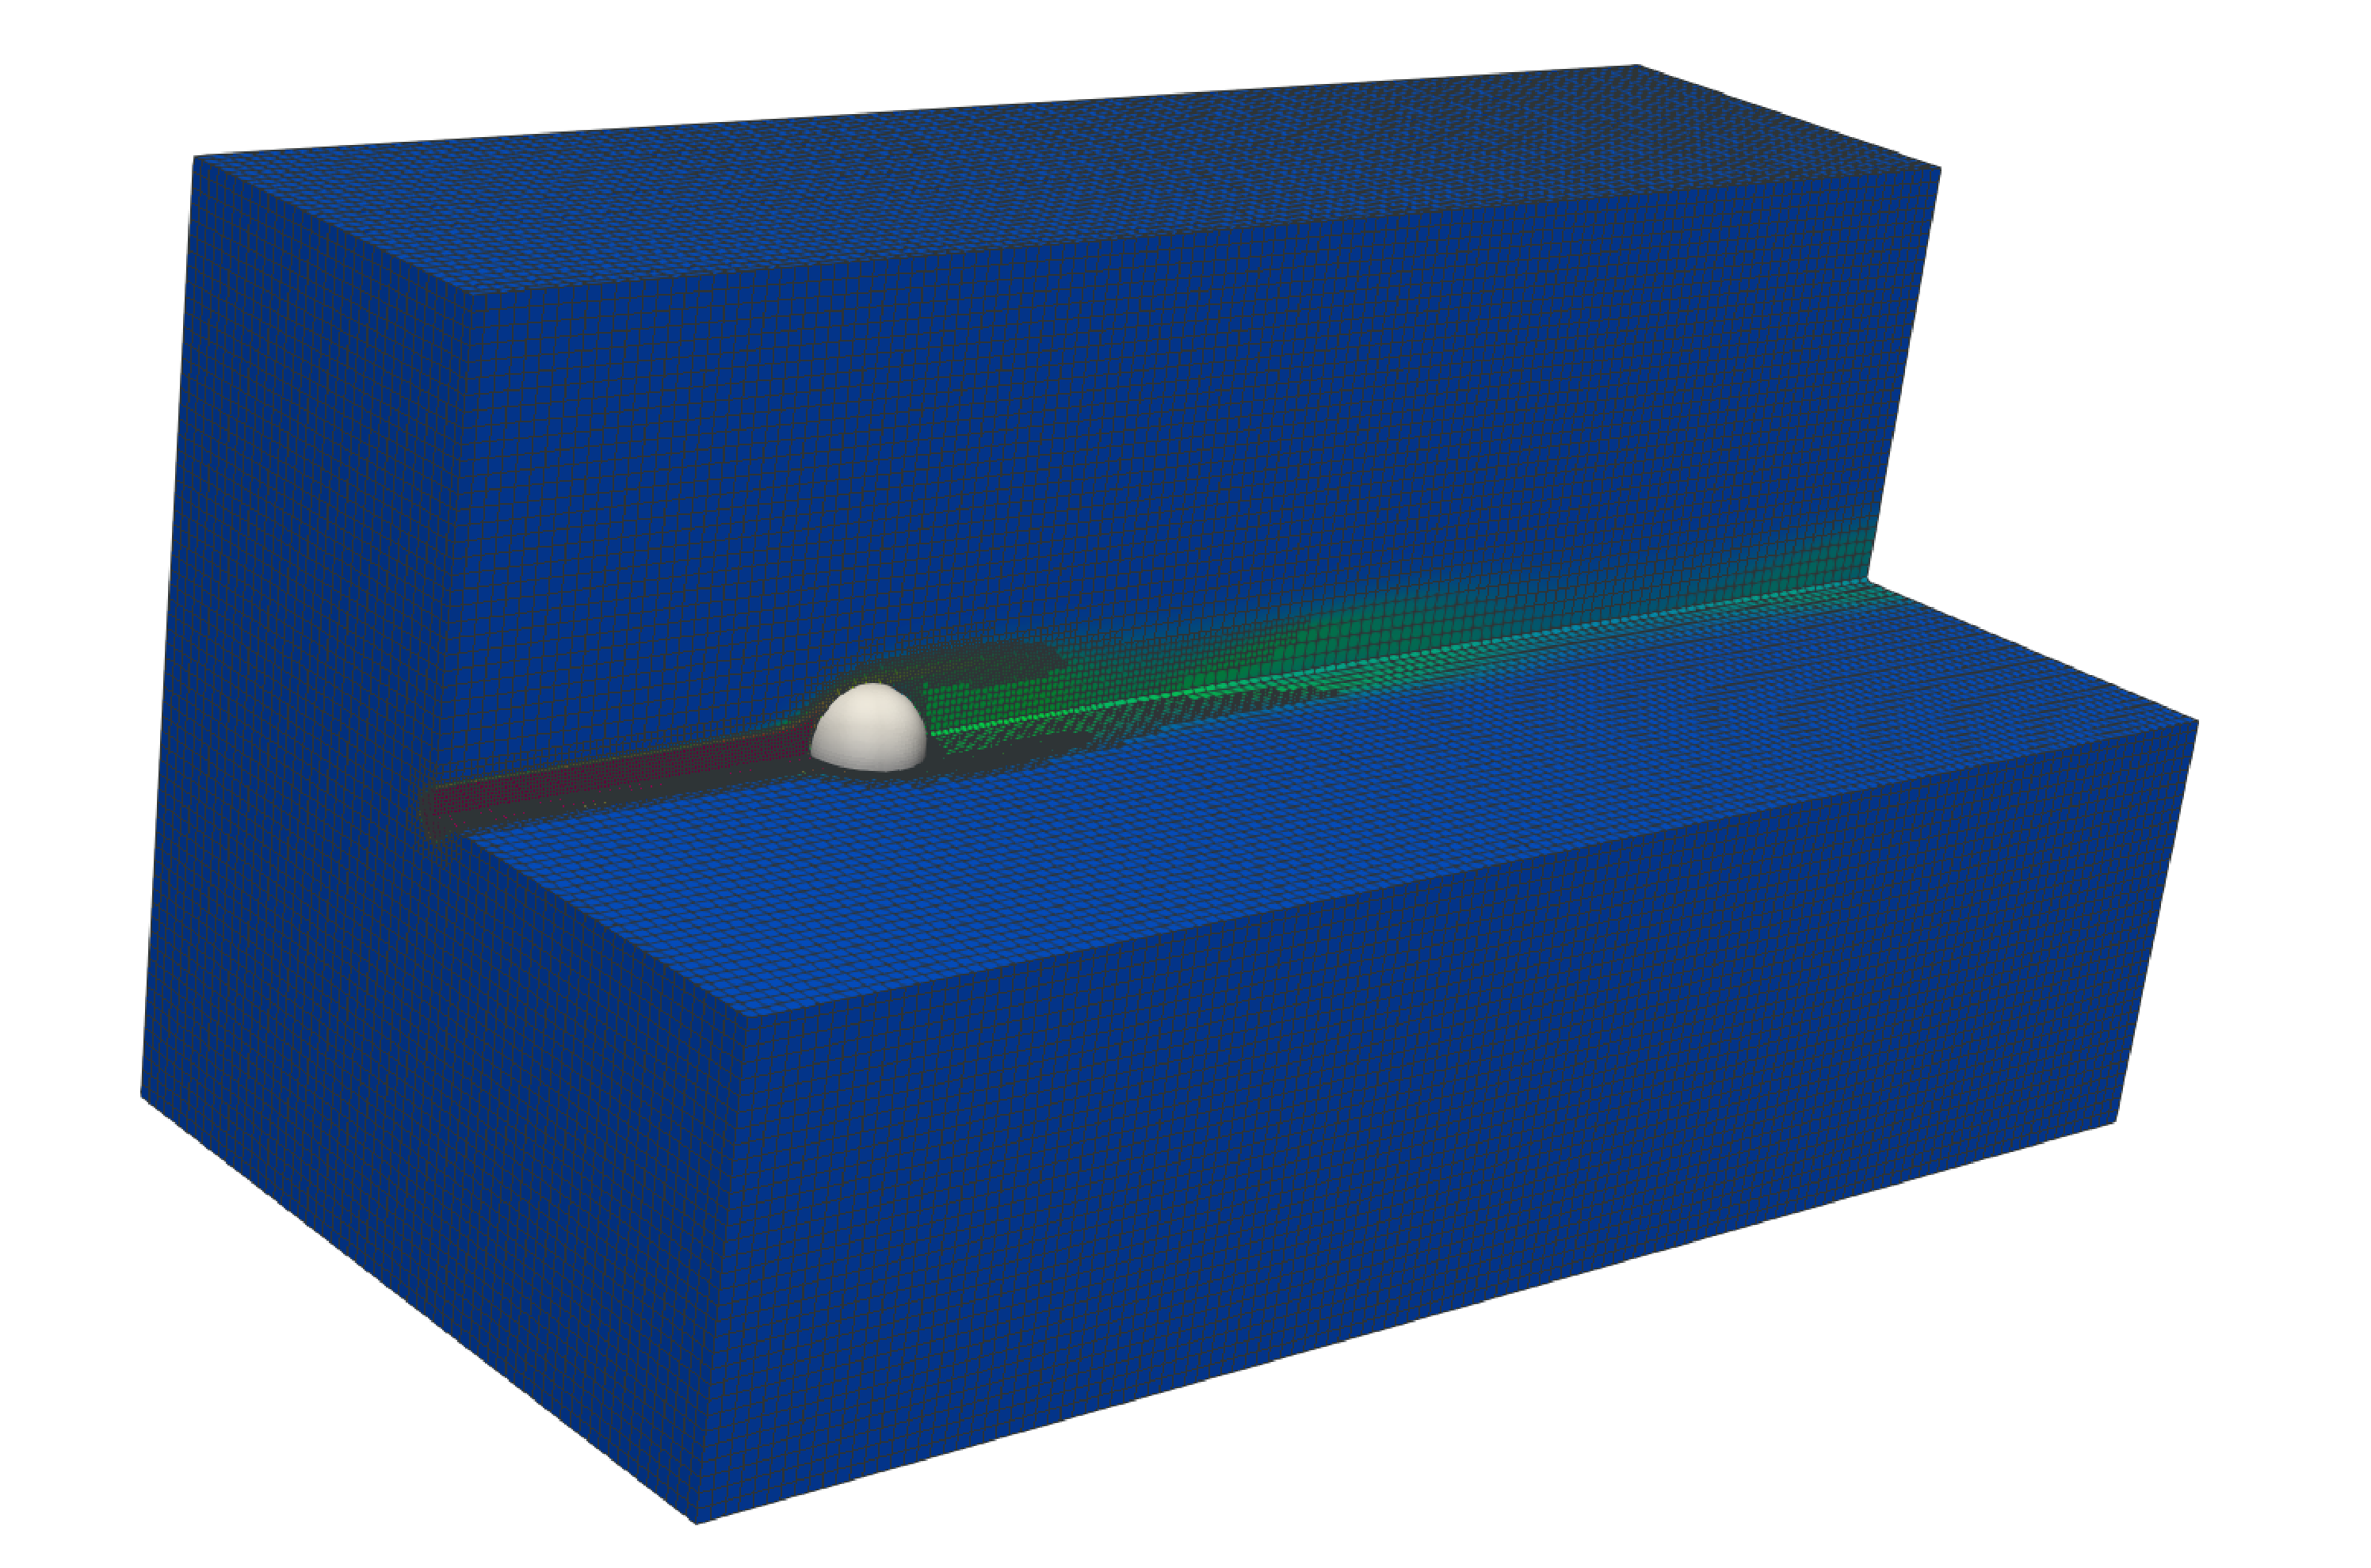
\includegraphics[width=0.95\textwidth]{./figures/flow_past_sphere/check_unchanged_behavior/original_grid_and_smoke_t_is_200.pdf} \\ 
  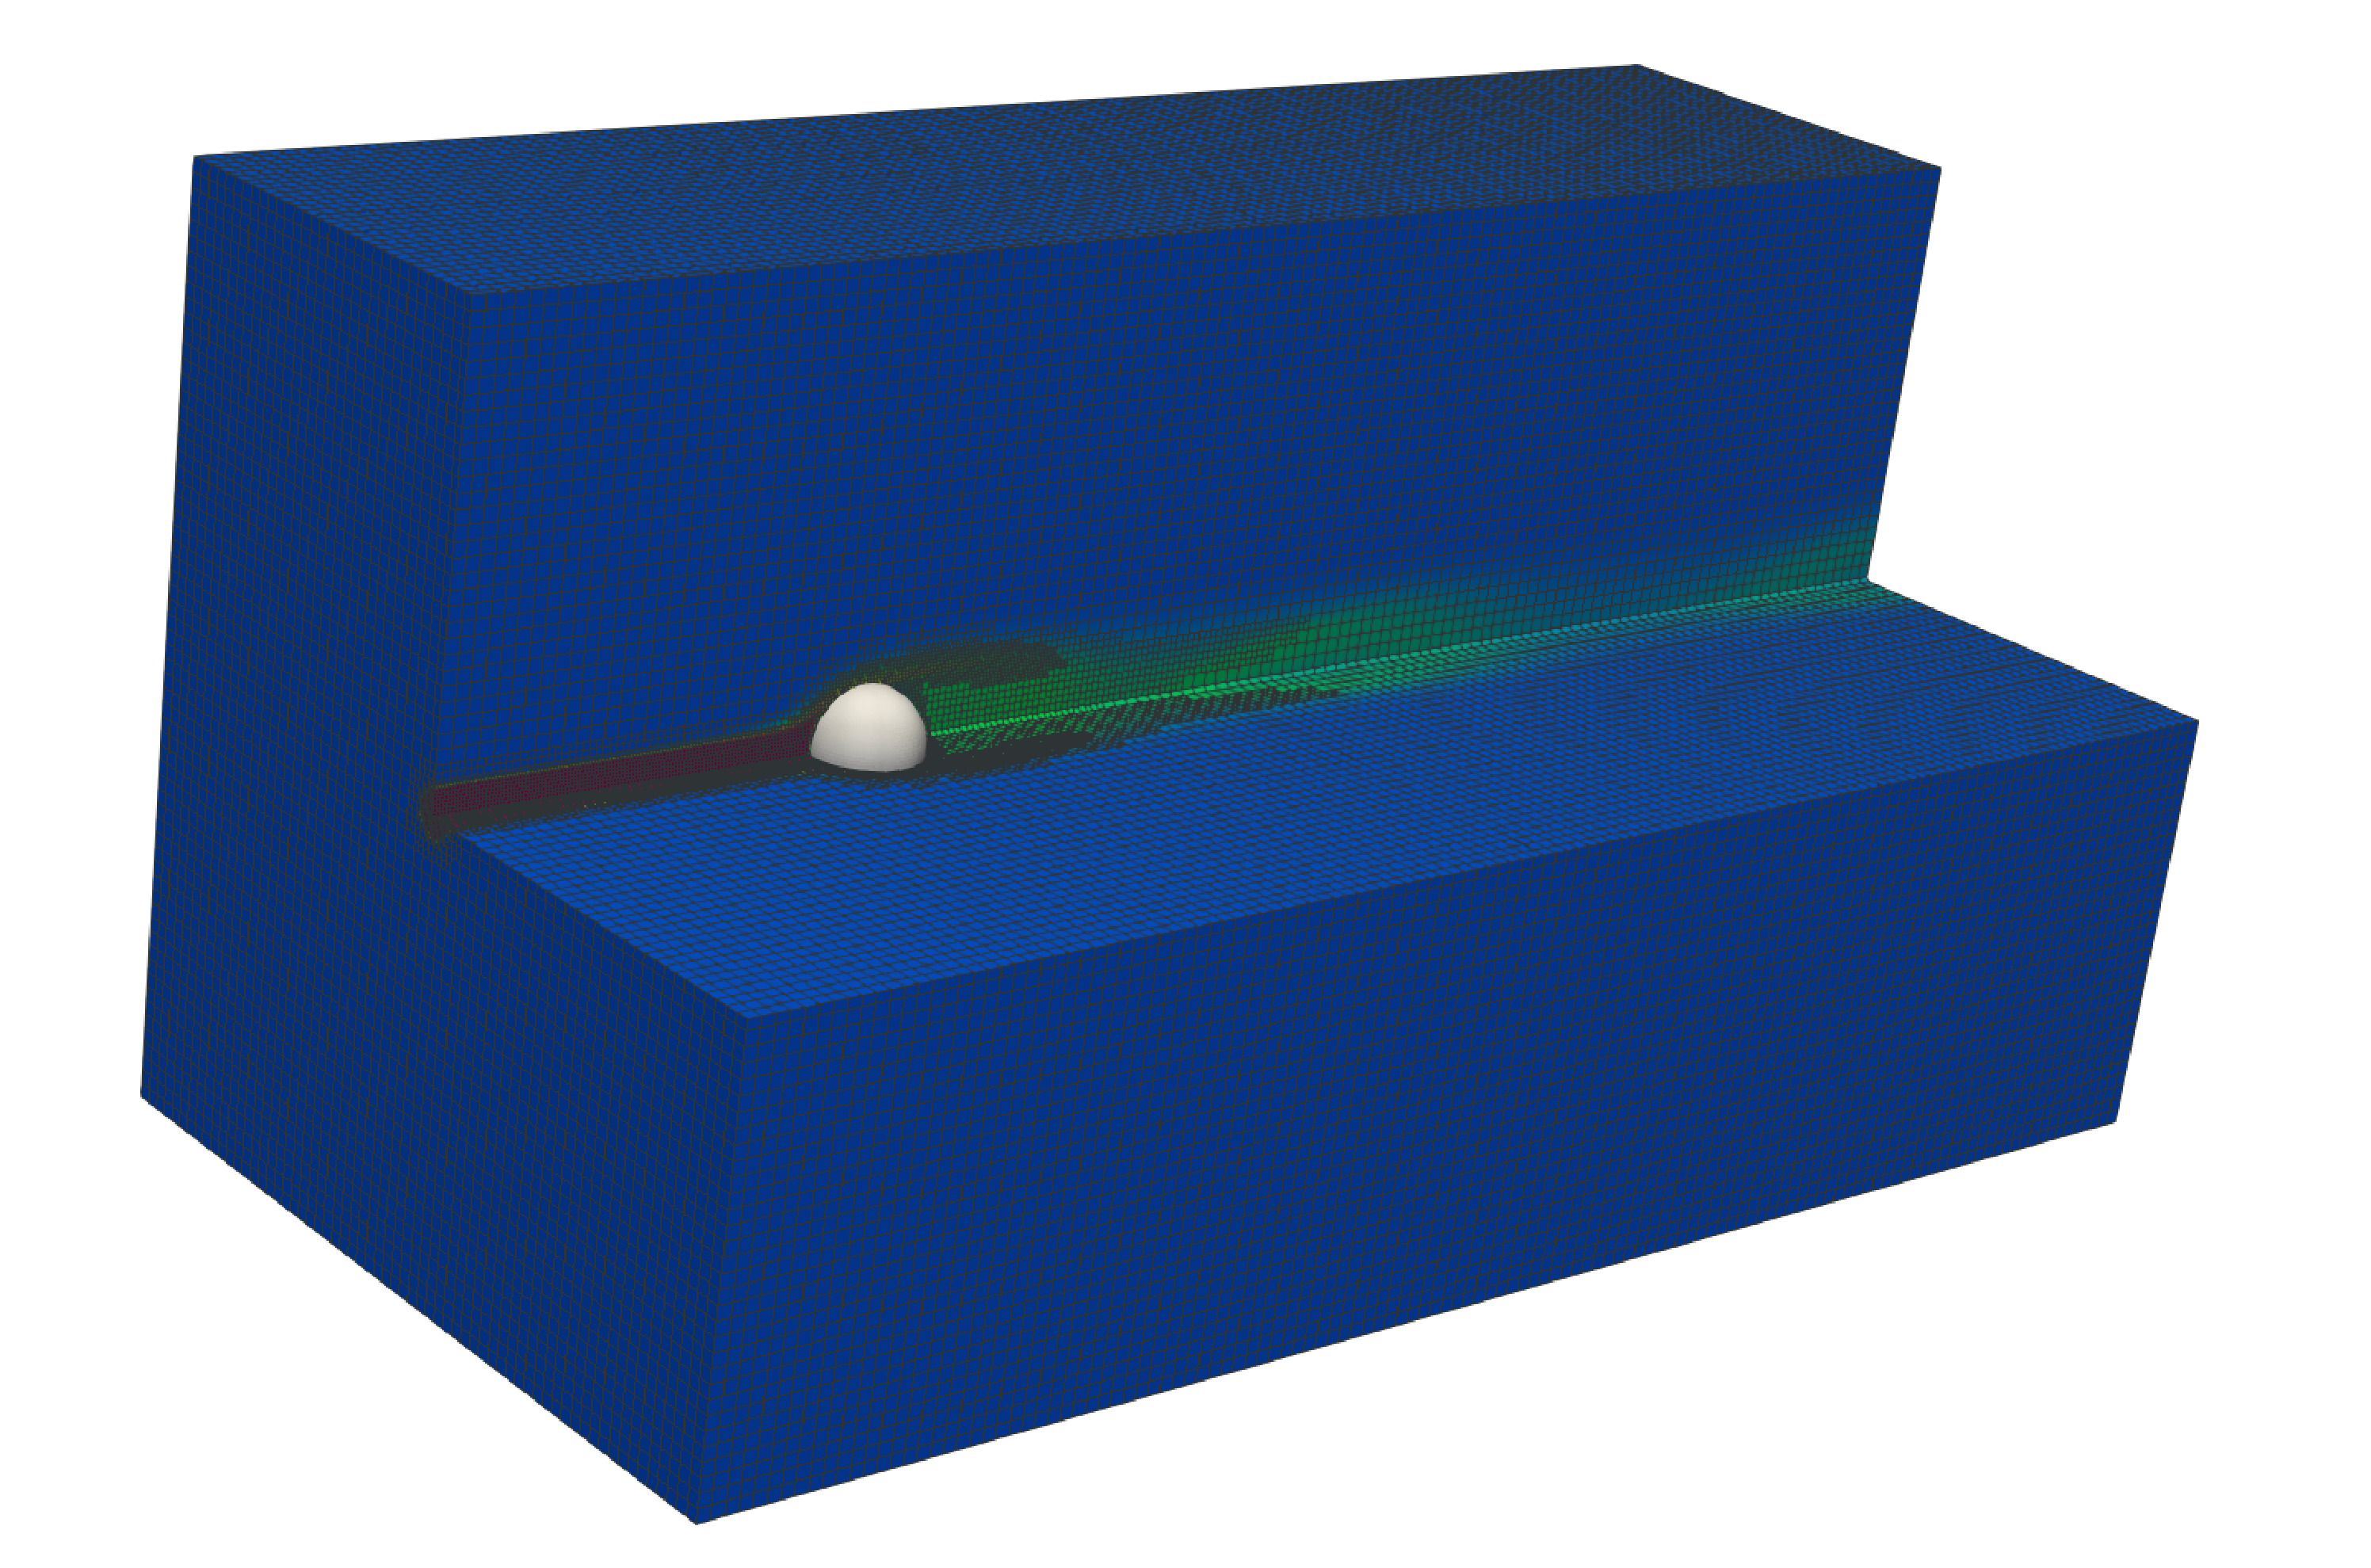
\includegraphics[width=0.95\textwidth]{./figures/flow_past_sphere/check_unchanged_behavior/optimized_grid_and_smoke_t_is_200.pdf}
 \caption{\label{fig:grid_and_smoke_flow_past_sphere_check_unchanged} computational grid and color map of the advected smoke for $t = 200$ in the simulation described in subsection \ref{subsec:flow_past_sphere_check}. Top: original solver; bottom: optimized solver.}
\end{figure}

\section{Assessment of newly added features departing from the original solver}
In this section, we present and investigate other features that were added to the Navier-Stokes solver to possibly accelerate its execution. In particular, we consider the possibility to re-use the cell and face solvers with appropriate good initial guesses within the inner loop and for successive time steps (if the grid has not changed, the interface has not moved and the boundary conditions have not changed). Concurrently, we consider the possibility to restrict the number of grid updates: given that the cylinder/sphere is static, we can take advantage of the constant physical description of the problem. 

\subsection{Flow past a cylinder with smoke and smoke-based refinement}
\label{subsec:assessment_cylinder_and_smoke}
For this analysis, we consider the same benchmark test case as described in subsection \ref{subsec:flow_past_cylinder_check}. However, instead of deleting the cell and face solvers right every single usage, the Navier-Stokes solver is now allowed to re-use cell and face solvers. We also increase the number of time steps between each grid update from $1$ to $2$, $4$ and $8$. 

When using the same solvers and the same preconditioners as originally hard-coded within the Navier-Stokes solver, \textit{i.e.}, \verb|BiCGStab| solvers for both the velocity components and the Hodge variable with \verb|SOR| preconditioning), the execution time drops to \SI{53}{\minute}\,\SI{48}{\second}, \SI{44}{\minute}\,\SI{27}{\second}, \SI{37}{\minute}\,\SI{56}{\second} and \SI{32}{\minute}\,\SI{3}{\second} when updating the grid every $1$, $2$, $4$ and $8$ time step(s) respectively. The gain in execution time when the grid is updated at every time step comes mainly from reusing the cell and face solvers as well as their preconditioners with good initial guesses within the inner loop for convergence of the Hodge variable. In this case, the gain is very small, which can be explained by the very small cost of building a \verb|SOR| preconditoner and the large number of iterations required by the Krylov subspace solvers to converge when using such a preconditioner. The force components over the time period $300 < t < 400$ are illustrated in \fig \ref{fig:forces_flow_past_cylinder_reused_solvers_bcgs_and_pcsor}. A time shit in the force results appears when the grid updates are prevented from happening at every time step, however the frequency of the vortex shedding does not seem to be affected.

When using a Conjugate Gradient (\verb|CG|) solver for the Hoge variable (the linear system to be solved is symmetric positive definite in this case) and \verb|HYPRE| preconditioners instead, the execution time drops to \SI{48}{\minute}\,\SI{52}{\second}, \SI{37}{\minute}\,\SI{39}{\second}, \SI{31}{\minute}\,\SI{3}{\second} and \SI{26}{\minute}\,\SI{18}{\second} when updating the grid every $1$, $2$, $4$ and $8$ time step(s), respectively. When compared to the results obtained with the original (hardcoded) solvers, this shows that one can gain even more execution time by using better suited solvers along with optimal preconditioners\footnote{Although costly to build, the \texttt{HYPRE} preconditioner is \emph{optimal} in several ways: the number of iterations required for convergence is significantly smaller than for most other available (parallel) preconditioners and it is also almost independent under further grid refinement (very efficient clustering).}. The force components over the time period $300 < t < 400$ are illustrated in \fig \ref{fig:forces_flow_past_cylinder_reused_solvers_cg_and_hypre}: note the similarity between graphs from \fig \ref{fig:forces_flow_past_cylinder_reused_solvers_bcgs_and_pcsor} and and graphs from \fig \ref{fig:forces_flow_past_cylinder_reused_solvers_cg_and_hypre}. 

\begin{figure}
  \centering
  \includegraphics[width=0.49\textwidth]{./results/flow_past_cylinder_smoke/optimized_run_reused_solvers_bcgs_and_pcsor/grid_update_1/force_history.pdf}
  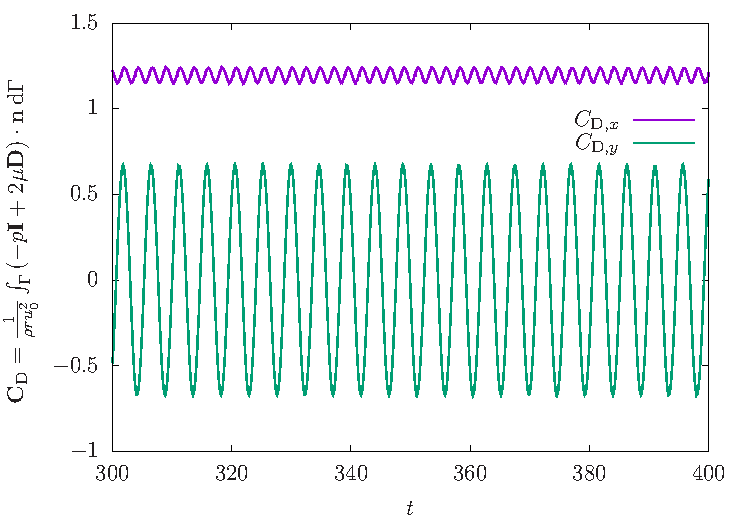
\includegraphics[width=0.49\textwidth]{./results/flow_past_cylinder_smoke/optimized_run_reused_solvers_bcgs_and_pcsor/grid_update_2/force_history.pdf} \\
  \includegraphics[width=0.49\textwidth]{./results/flow_past_cylinder_smoke/optimized_run_reused_solvers_bcgs_and_pcsor/grid_update_4/force_history.pdf} 
  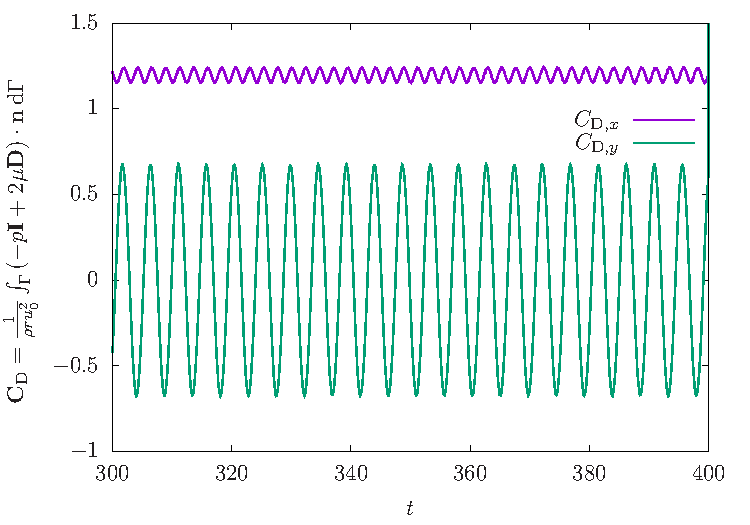
\includegraphics[width=0.49\textwidth]{./results/flow_past_cylinder_smoke/optimized_run_reused_solvers_bcgs_and_pcsor/grid_update_8/force_history.pdf} \\
 \caption{\label{fig:forces_flow_past_cylinder_reused_solvers_bcgs_and_pcsor} history of the non-dimensional force components for $300 < t < 400$ in the simulation described in subsection \ref{subsec:flow_past_cylinder_check}. These results have been obtained with \texttt{BiCGStab} solvers for the velocity components and the Hodge variable. All solvers are preconditioned using \texttt{SOR} preconditioning. The solvers and their preconditioners are re-used as long as they are valid. The grid is updated every $1$, $2$, $4$ and $8$ time step(s), from top left to bottom right figure.} 
\end{figure}

\begin{figure}
  \centering
  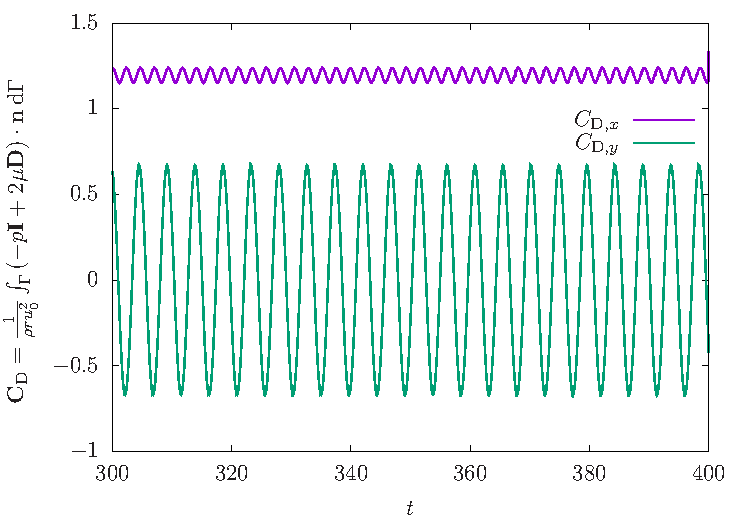
\includegraphics[width=0.49\textwidth]{./results/flow_past_cylinder_smoke/optimized_run_reused_solvers_cg_and_pchypre/grid_update_1/force_history.pdf} 
  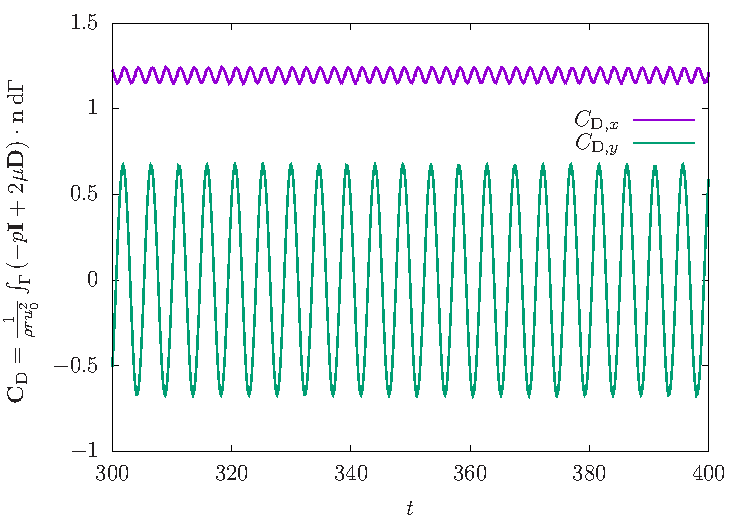
\includegraphics[width=0.49\textwidth]{./results/flow_past_cylinder_smoke/optimized_run_reused_solvers_cg_and_pchypre/grid_update_2/force_history.pdf} \\
  \includegraphics[width=0.49\textwidth]{./results/flow_past_cylinder_smoke/optimized_run_reused_solvers_cg_and_pchypre/grid_update_4/force_history.pdf}
  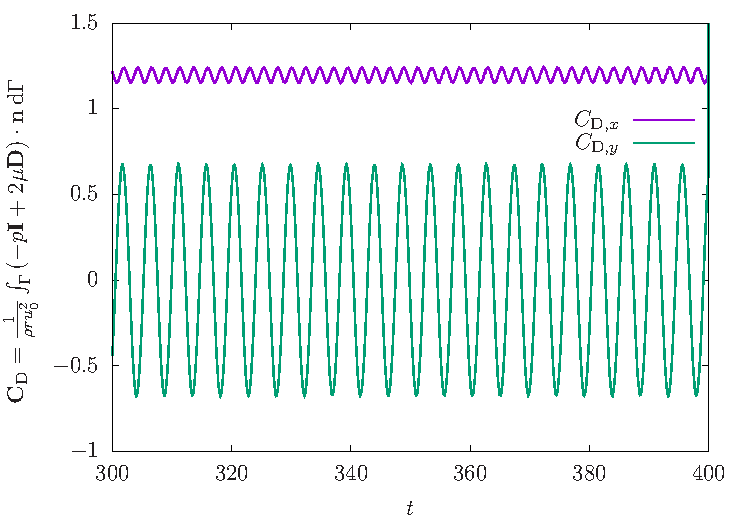
\includegraphics[width=0.49\textwidth]{./results/flow_past_cylinder_smoke/optimized_run_reused_solvers_cg_and_pchypre/grid_update_8/force_history.pdf} \\
 \caption{\label{fig:forces_flow_past_cylinder_reused_solvers_cg_and_hypre} history of the non-dimensional force components for $300 < t < 400$ in the simulation described in subsection \ref{subsec:flow_past_cylinder_check}. These results have been obtained with a \texttt{CG} solver for the Hodge variable and \texttt{BiCGStab} solvers for the velocity components. All solvers are preconditioned using the \texttt{HYPRE} preconditioner. The solvers and their preconditioners are re-used as long as they are valid. The grid is updated every (from top left to bottom right figure): $1$ time step, $2$ time steps, $4$ time steps, $8$ time steps.} 
\end{figure}


\subsection{Flow past a sphere with smoke and smoke-based refinement}
\label{subsec:assessment_sphere_and_smoke}
For this analysis, we consider the same benchmark test case as described in subsection \ref{subsec:flow_past_sphere_check}. However, instead of deleting the cell and face solvers right every single usage, the Navier-Stokes solver is now allowed to re-use cell and face solvers. We also increase the number of time steps between each grid update from $1$ to $2$, $4$ and $8$. 

When using the same solvers and the same preconditioners as originally hard-coded within the Navier-Stokes solver, \textit{i.e.}, \verb|BiCGStab| solvers for both the velocity components and the Hodge variable with \verb|SOR| preconditioning), the execution time drops to \SI{20}{\hour}\,\SI{32}{\minute}\,\SI{32}{\second}, \SI{13}{\hour}\,\SI{30}{\minute}\,\SI{52}{\second}, \SI{10}{\hour}\,\SI{18}{\minute}\,\SI{41}{\second} and \SI{8}{\hour}\,\SI{26}{\minute}\,\SI{31}{\second} when updating the grid every $1$, $2$, $4$ and $8$ time step(s) respectively. In this case, the gain is much more significant than in the two-dimensional case when solvers are reused, and can probably be explained by a significant reduction in the number of iterations required by the iterative solvers for convergence, when the Krylov solvers start from good initial guesses. The force components over the time period $100 < t < 200$ are illustrated in \fig \ref{fig:forces_flow_past_sphere_reused_solvers_bcgs_and_pcsor}. A time shit in the force results appears when the grid updates are prevented from happening at every time step, however the frequency of the vortex shedding does not seem to be affected.

When using a Conjugate Gradient (\verb|CG|) solver for the Hoge variable (the linear system to be solved is symmetric positive definite in this case) along with a \verb|HYPRE| preconditioner for the cell-solver\footnote{The linear systems for the face problems have a significant positive diagonal contribution and only a few iterations are required for convergence even with simple \texttt{SOR} preconditioners, it does not seem relevant to consider another kind of costly-to-build conditioner for threse problems} instead, the execution time drops to \SI{20}{\hour}\,\SI{44}{\minute}\,\SI{48}{\second}, \SI{14}{\hour}\,\SI{6}{\minute}\,\SI{54}{\second}, \SI{10}{\hour}\,\SI{4}{\minute}\,\SI{43}{\second} and \SI{8}{\hour}\,\SI{20}{\minute}\,\SI{40}{\second} when updating the grid every $1$, $2$, $4$ and $8$ time step(s), respectively. Contrary to the two-dimensional case, it seems like the complexity of building the \verb|HYPRE| preconditioner takes over when assessing the computational cost of solving the linear systems in this case: one gains execution time only when grid updates are prevented (allowing more reuse of the costly-to-build preconditioner). No general conclusion can be drawn from these results however since solver performances are case- and eigenvalues-dependent\footnote{Personally, I expect \texttt{HYPRE} to outperform \texttt{SOR} preconditioning when dealing with larger and finer grids because of the larger spectrum of eigenvalues to be clustered.}. 

The force components over the time period $100 < t < 200$ are illustrated in \fig \ref{fig:forces_flow_past_sphere_reused_solvers_cg_and_hypre}: note the similarity between graphs from \fig \ref{fig:forces_flow_past_sphere_reused_solvers_bcgs_and_pcsor} and graphs from \fig \ref{fig:forces_flow_past_sphere_reused_solvers_cg_and_hypre}. 

\begin{figure}
  \centering
  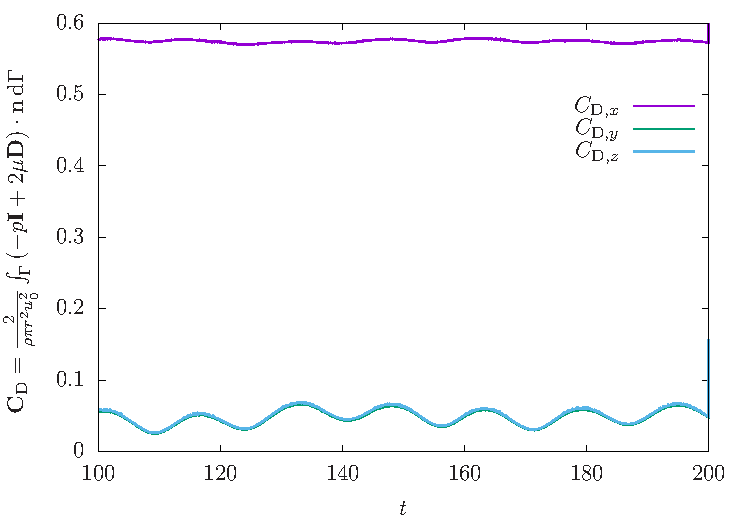
\includegraphics[width=0.49\textwidth]{./results/flow_past_sphere_smoke/optimized_run_reused_solvers_bcgs_and_pcsor/grid_update_1/force_history.pdf} 
  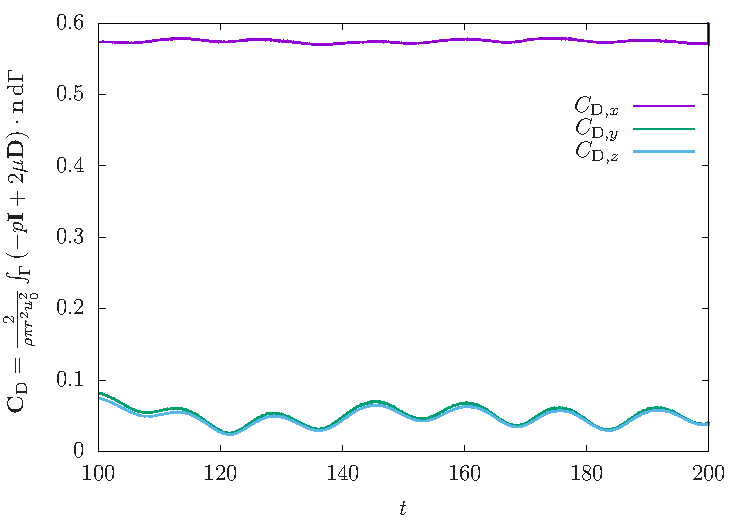
\includegraphics[width=0.49\textwidth]{./results/flow_past_sphere_smoke/optimized_run_reused_solvers_bcgs_and_pcsor/grid_update_2/force_history.pdf} \\
  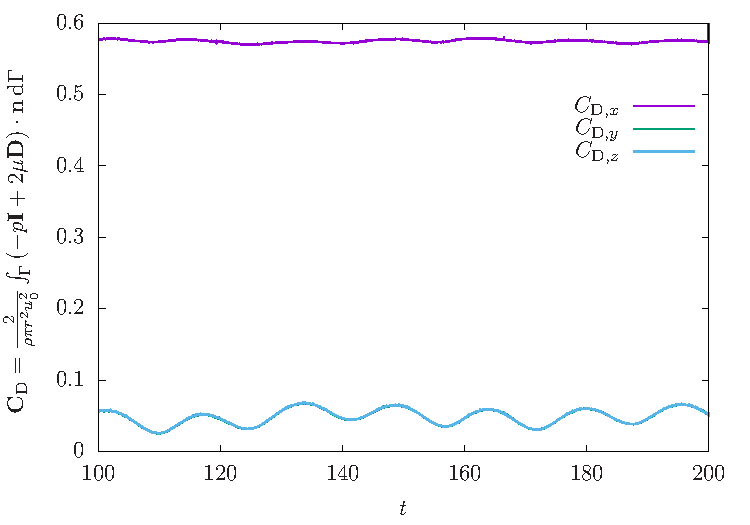
\includegraphics[width=0.49\textwidth]{./results/flow_past_sphere_smoke/optimized_run_reused_solvers_bcgs_and_pcsor/grid_update_4/force_history.pdf}
  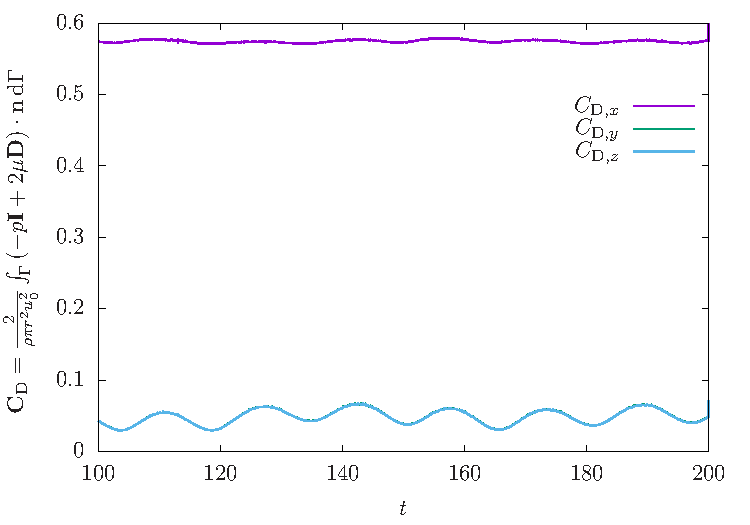
\includegraphics[width=0.49\textwidth]{./results/flow_past_sphere_smoke/optimized_run_reused_solvers_bcgs_and_pcsor/grid_update_8/force_history.pdf} \\
 \caption{\label{fig:forces_flow_past_sphere_reused_solvers_bcgs_and_pcsor} history of the non-dimensional force components for $100 < t < 200$ in the simulation described in subsection \ref{subsec:flow_past_sphere_check}. These results have been obtained with \texttt{BiCGStab} solvers for the velocity components and the Hodge variable. All solvers are preconditioned using \texttt{SOR} preconditioning. The solvers and their preconditioners are re-used as long as they are valid. The grid is updated every $1$, $2$, $4$ and $8$ time step(s), from top left to bottom right figure. The sign of the results for the $y$- and $z$- components was inverted in the top right figure, for comparison purposes.} 
\end{figure}

\begin{figure}
  \centering
  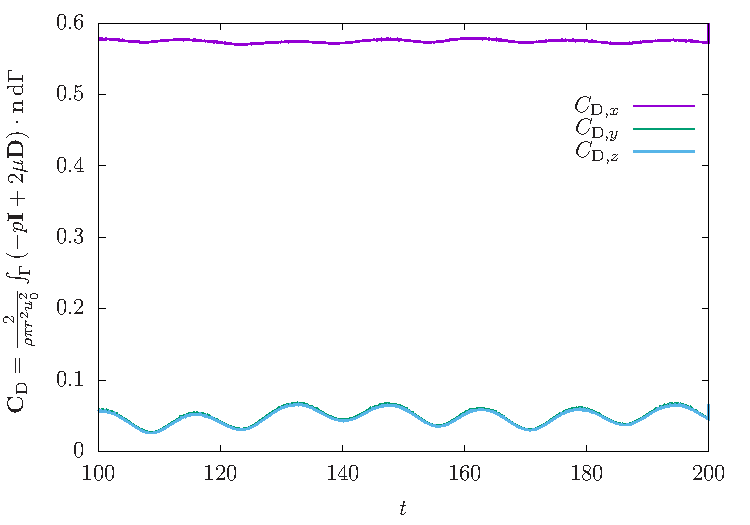
\includegraphics[width=0.49\textwidth]{./results/flow_past_sphere_smoke/optimized_run_reused_solvers_cg_and_pchypre/grid_update_1/force_history.pdf}
  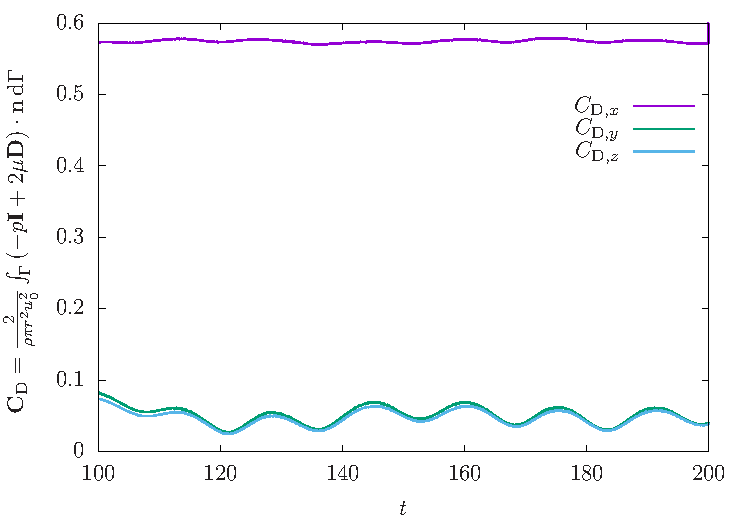
\includegraphics[width=0.49\textwidth]{./results/flow_past_sphere_smoke/optimized_run_reused_solvers_cg_and_pchypre/grid_update_2/force_history.pdf} \\
  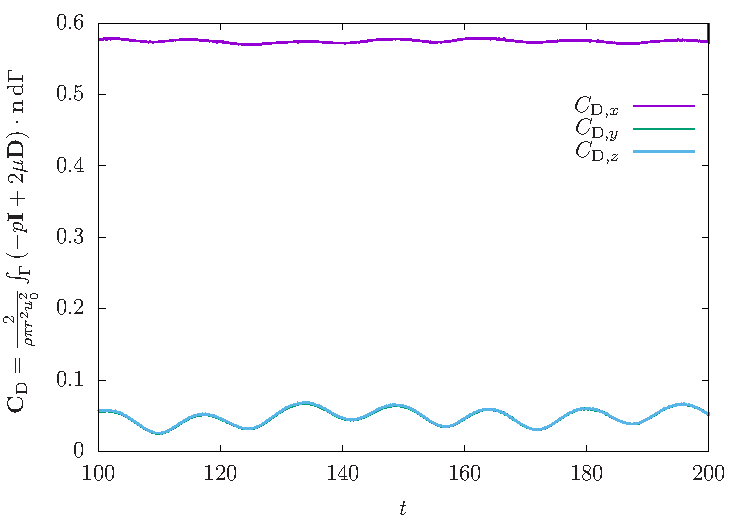
\includegraphics[width=0.49\textwidth]{./results/flow_past_sphere_smoke/optimized_run_reused_solvers_cg_and_pchypre/grid_update_4/force_history.pdf} 
  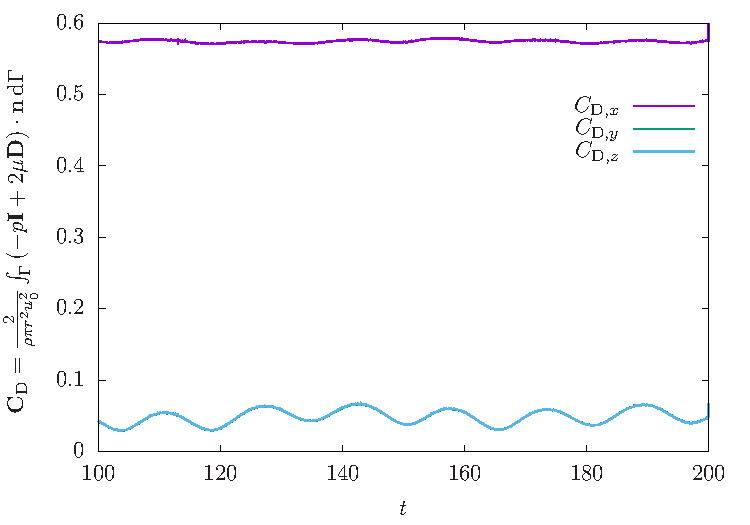
\includegraphics[width=0.49\textwidth]{./results/flow_past_sphere_smoke/optimized_run_reused_solvers_cg_and_pchypre/grid_update_8/force_history.pdf} \\
 \caption{\label{fig:forces_flow_past_sphere_reused_solvers_cg_and_hypre} history of the non-dimensional force components for $100 < t < 200$ in the simulation described in subsection \ref{subsec:flow_past_sphere_check}. These results have been obtained with a \texttt{CG} solver for the Hodge variable and \texttt{BiCGStab} solvers for the velocity components. The \texttt{CG} solver is preconditioned with the \texttt{HYPRE} preconditioner while the \texttt{BiCGStab} solvers are preconditioned using \texttt{SOR} preconditioners. The solvers and their preconditioners are re-used as long as they are valid. The grid is updated every (from top left to bottom right figure): $1$ time step, $2$ time steps, $4$ time steps, $8$ time steps, from top left to bottom right figure. Here again, the sign of the results for the $y$- and $z$- components was inverted in the top right figure, for comparison purposes.} 
\end{figure} 


\section{A note on a possible change of behavior}

Finally, we want to assess and evaluate the possible change of behavior of the solver, in \emph{absence} of grid refinement based on a passively advected scalar. Indeed, the iterative grid update procedure was modified in order to avoid the (costly) creation of ghost layers for every iterative step. As detailed in subsection \ref{subsec:nonrestricted_optimization_of_the_solver}, this modification \emph{might} induce a very slight change of behavior in the solver: if the node value triggering the refinement criterion happens to be a T-junction at the border of the domain's partition but owned by another processor, this node would be missed locally and would not trigger local refinement. However, we expect that to be relatively rare and mitigated by the grid repartitioning (within the iterative process) and the 2:1 grid balancing.

In order to assess that possibility, we compared the original and optimized solver on the same test case as described in subsection \ref{subsec:flow_past_sphere_check}, but \emph{without} passive advection. For the entire run, the only difference observed in the exported results relates to slight differences in the very first residuals for the Hodge variable in $3$ out of $3,852$ time steps. These slight differences can be explained by a modification brought to the Moving-Least-Square cell-interpolation procedure that intends to make the procedure more robust and less sensitive to the grid size (comparison of dimensionally consistent double-precision real numbers). No difference in computational grids is reported, so the solver's behavior was not affected by the modified strategy.

In terms of performance, the original solver completed the simulation in \SI{1}{\day}\,\SI{9}{\hour}\,\SI{30}{\minute}\,\SI{4}{\second} while the optimized solver completed the very same task with the exact same numerics in \SI{22}{\hour}\,\SI{51}{\minute}\,\SI{30}{\second}, that is a \textbf{31.77\% gain}.

\begin{figure}
  \centering
  \includegraphics[width=0.49\textwidth]{./results/flow_past_sphere_smoke/reference/force_history.pdf}
  \includegraphics[width=0.49\textwidth]{./results/flow_past_sphere_smoke/optimized_run/force_history.pdf}
 \caption{\label{fig:forces_flow_past_sphere_check_unchanged} history of the non-dimensional force components for $100 < t < 200$ in the simulation described in subsection \ref{subsec:flow_past_sphere_check}. Top: original solver; bottom: optimized solver. (The graphs for $C_{\mathrm{D}, y}$ and $C_{\mathrm{D}, z}$ overlap)} 
\end{figure}

\newpage
\section{Summary}
The results of the optimization analyses are summarized in Tables \ref{tab:flow_past_cylinder_with_smoke} and \ref{tab:flow_past_sphere_with_smoke}.

\begin{landscape}

\begin{table}
  \newcommand{\mc}[3]{\multicolumn{#1}{#2}{#3}}
  \begin{center}
    \begin{tabular}[t]{|c|c|c|c|p{10mm}|p{25mm}|c|c|p{55mm}|}\hline
      N-S solver & cell-solver & face-solver & precond. & solver re-use & \mc{1}{c|}{grid update} & execution time & gain & \mc{1}{c|}{notes}\\\hhline{|=|=|=|=|=|=|=|=|=|}
      original & \verb|BiCGStab| & \verb|BiCGStab| & SOR & \mc{1}{c|}{no} & every time step & \SI{1}{\hour}\,\SI{41}{\minute}\,\SI{45}{\second} & 0\% & reference results (before significant code changes) \\\hline
      optimized & \verb|BiCGStab| & \verb|BiCGStab| & SOR & \mc{1}{c|}{no} & every time step & \SI{56}{\minute}\,\SI{19}{\second} & 44.64\% & exact same results except for a few initial residuals of the Hodge variable ($6$ out of $9,950$ time steps)\\\hhline{|=|=|=|=|=|=|=|=|=|}
      optimized & \verb|BiCGStab| & \verb|BiCGStab| & SOR & \mc{1}{c|}{yes} & every time step & \SI{53}{\minute}\,\SI{48}{\second} & 47.13\% & same numerics as originally, results are almost exactly the same \\\hline
      optimized & \verb|BiCGStab| & \verb|BiCGStab| & SOR & \mc{1}{c|}{yes} & once every $2$ time steps & \SI{44}{\minute}\,\SI{27}{\second} & 56.31\% & time shift but frequency of vortex shedding unchanged\\\hline
      optimized & \verb|BiCGStab| & \verb|BiCGStab| & SOR & \mc{1}{c|}{yes} & once every $4$ time steps & \SI{37}{\minute}\,\SI{56}{\second} & 62.72\% & same as above \\\hline
      optimized & \verb|BiCGStab| & \verb|BiCGStab| & SOR & \mc{1}{c|}{yes} & once every $8$ time steps & \SI{32}{\minute}\,\SI{3}{\second}  & 68.5\% & same as above \\\hhline{|=|=|=|=|=|=|=|=|=|}
      optimized & CG & \verb|BiCGStab| & \verb|HYPRE| & \mc{1}{c|}{yes} & every time step           & \SI{48}{\minute}\,\SI{52}{\second} & 51.97\% & different numerics than originally, but results are almost exactly the same \\\hline
      optimized & CG & \verb|BiCGStab| & \verb|HYPRE| & \mc{1}{c|}{yes} & once every $2$ time steps & \SI{37}{\minute}\,\SI{39}{\second} & 63.00\% & time shift but frequency of vortex shedding unchanged \\\hline
      optimized & CG & \verb|BiCGStab| & \verb|HYPRE| & \mc{1}{c|}{yes} & once every $4$ time steps & \SI{31}{\minute}\,\SI{3}{\second} & 69.48 \% & same as above \\\hline
      optimized & CG & \verb|BiCGStab| & \verb|HYPRE| & \mc{1}{c|}{yes} & once every $8$ time steps & \SI{26}{\minute}\,\SI{18}{\second} & 74.15\% & same as above \\\hline
    \end{tabular}
  \end{center}
  \caption{\label{tab:flow_past_cylinder_with_smoke} summary of the runtime-optimization results for two-dimensional flow past a cylinder with advection of smoke and smoke-based grid refinement.}
\end{table}

\begin{table}
  \newcommand{\mc}[3]{\multicolumn{#1}{#2}{#3}}
  \begin{center}
    \begin{tabular}[t]{|c|c|c|c|p{10mm}|p{25mm}|c|c|p{55mm}|}\hline
      N-S solver & cell-solver & face-solver & precond. & solver re-use & \mc{1}{c|}{grid update} & execution time & gain & \mc{1}{c|}{notes}\\\hhline{|=|=|=|=|=|=|=|=|=|}
      original & \verb|BiCGStab| & \verb|BiCGStab| & SOR & \mc{1}{c|}{no} & every time step &  \SI{1}{\day}\,\SI{11}{\hour}\,\SI{12}{\minute}\,\SI{56}{\second} & 0\% & reference results (before significant code changes) \\\hline
      optimized & \verb|BiCGStab| & \verb|BiCGStab| & SOR & \mc{1}{c|}{no} & every time step & \SI{23}{\hour}\,\SI{12}{\minute}\,\SI{41}{\second} & 34.09\% & exact same results except for a few initial residuals of the Hodge variable ($6$ out of $3,852$ time steps)\\\hhline{|=|=|=|=|=|=|=|=|=|}
      optimized & \verb|BiCGStab| & \verb|BiCGStab| & SOR & \mc{1}{c|}{yes} & every time step & \SI{20}{\hour}\,\SI{32}{\minute}\,\SI{32}{\second} & 41.67\% & similar numerics as above, results are almost exactly the same \\\hline
      optimized & \verb|BiCGStab| & \verb|BiCGStab| & SOR & \mc{1}{c|}{yes} & once every $2$ time steps & \SI{13}{\hour}\,\SI{30}{\minute}\,\SI{52}{\second} & 61.62\% & time shift but frequency of vortex shedding unchanged (sign inversion for $y$ and $z$)\\\hline
      optimized & \verb|BiCGStab| & \verb|BiCGStab| & SOR & \mc{1}{c|}{yes} & once every $4$ time steps & \SI{10}{\hour}\,\SI{18}{\minute}\,\SI{41}{\second} & 70.72\% & same as above (no sign inversion) \\\hline
      optimized & \verb|BiCGStab| & \verb|BiCGStab| & SOR & \mc{1}{c|}{yes} & once every $8$ time steps & \SI{8}{\hour}\,\SI{26}{\minute}\,\SI{31}{\second} & 76.03\% & same as above (no sign inversion) \\\hhline{|=|=|=|=|=|=|=|=|=|}
      optimized & CG & \verb|BiCGStab| & \verb|HYPRE| & \mc{1}{c|}{yes} & every time step           & \SI{20}{\hour}\,\SI{44}{\minute}\,\SI{48}{\second} & 41.09\% & different numerics than originally, but results are almost exactly the same \\\hline
      optimized & CG & \verb|BiCGStab| & \verb|HYPRE| & \mc{1}{c|}{yes} & once every $2$ time steps & \SI{14}{\hour}\,\SI{6}{\minute}\,\SI{54}{\second} & 59.92\% & time shift but frequency of vortex shedding unchanged (sign inversion for $y$ and $z$) \\\hline
      optimized & CG & \verb|BiCGStab| & \verb|HYPRE| & \mc{1}{c|}{yes} & once every $4$ time steps & \SI{10}{\hour}\,\SI{4}{\minute}\,\SI{43}{\second} & 71.38\% & same as above (no sign inversion) \\\hline
      optimized & CG & \verb|BiCGStab| & \verb|HYPRE| & \mc{1}{c|}{yes} & once every $8$ time steps & \SI{8}{\hour}\,\SI{20}{\minute}\,\SI{40}{\second} & 76.30\% & same as above (no sign inversion) \\\hline
    \end{tabular}
  \end{center}
  \caption{\label{tab:flow_past_sphere_with_smoke} summary of the runtime-optimization results for three-dimensional flow past a sphere with advection of smoke and smoke-based grid refinement. When the \texttt{HYPRE} preconditioner is used, it is only for the cell solver. }
\end{table}
\end{landscape}


\end{document}




